\documentclass[sigplan,10pt,review,anonymous]{acmart}\settopmatter{printfolios=true,printccs=false,printacmref=false}

\usepackage{float}
\usepackage{amsmath,amssymb,amsfonts}
\usepackage[ruled, vlined]{algorithm2e}
\usepackage{graphicx}
\usepackage{textcomp}
\usepackage{xcolor}
\usepackage{listings}
\usepackage{caption}
\usepackage{subcaption}
\usepackage{multirow}
\usepackage{booktabs}
\usepackage{makecell}
\usepackage{galois}
\usepackage{mathpartir}
\usepackage{bussproofs}
\usepackage{mathtools}

\EnableBpAbbreviations

\setcopyright{acmcopyright}
\copyrightyear{2018}
\acmYear{2018}
\acmDOI{10.1145/1122445.1122456}
\acmConference[Woodstock '18]{Woodstock '18: ACM Symposium on Neural
  Gaze Detection}{June 03--05, 2018}{Woodstock, NY}
\acmPrice{15.00}
\acmISBN{978-1-4503-XXXX-X/18/06}

% thicker vertical line
\newcolumntype{?}{!{\vrule width 1pt}}

% Styles
\definecolor{dkgreen}{rgb}{0,0.6,0}
\definecolor{gray}{rgb}{0.5,0.5,0.5}
\definecolor{mauve}{rgb}{0.58,0,0.82}
\lstdefinelanguage{JavaScript}{
  keywords={async, await, break, case, catch, class, const, continue, debugger,
    default, delete, do, else, enum, export, extends, false, finally, for,
    function, if, import, in, instanceof, new, null, return, super, switch, this,
    throw, true, try, typeof, var, void, while, with, yield},
  keywordstyle=\color{blue}\bfseries,
  ndkeywordstyle=\color{darkgray}\bfseries,
  identifierstyle=\color{black},
  sensitive=false,
  comment=[l]{//},
  morecomment=[s]{/*}{*/},
  commentstyle=\color{dkgreen}\ttfamily,
  stringstyle=\color{purple}\ttfamily,
  morestring=[b]',
  morestring=[b]"
}
\lstdefinestyle{myJSstyle}{
  language=JavaScript,
  numbers=left,
  stepnumber=1,
  extendedchars=true,
  basicstyle=\footnotesize\ttfamily,
  showstringspaces=false,
  showspaces=false,
  tabsize=2,
  breaklines=true,
  showtabs=false,
  captionpos=b
}

% Basic
\DeclareMathAlphabet{\mathpzc}{T1}{pzc}{m}{it}
\newcommand{\powerset}[1]{\mathcal{P}(#1)}
\newcommand{\imbox}[1]{\mbox{\small \textit{#1}}}
\newcommand{\name}[1]{\textsf{#1}}
\newcommand{\inred}[1]{{\color{red}{#1}}}
\newcommand{\todo}{\inred{TODO}}
\newcommand{\abs}[1]{{#1}^{\#}}
\newcommand{\finmap}{{\xrightarrow[]{\text{fin}}}}
\newcommand{\mapstos}{\;\dot{\mapsto}\;}
\newcommand{\Dom}{\name{Dom}}

% Tool
\newcommand{\tool}{\text{SAFE}_\name{DS}}

% Keywords
\newcommand{\jscode}[1]{\text{\lstinline[style=myJSstyle,numbers=none]!#1!}}
\newcommand{\code}[1]{\texttt{#1}}
\newcommand{\kwif}{\code{if}}
\newcommand{\kwelse}{\code{else}}
\newcommand{\kwret}{\code{ret}}
\newcommand{\kwobj}{\code{\{\}}}
\newcommand{\kwtrue}{\code{true}}
\newcommand{\kwfalse}{\code{false}}

% Notations
\newcommand{\prog}{P}
\newcommand{\labset}{\mathcal{L}}
\newcommand{\lab}{\mathpzc{l}}
\newcommand{\labdot}[1]{{{\bullet_{\lab_{#1}}}}}
\newcommand{\ilab}{\lab_\iota}
\newcommand{\labnext}{\name{next}}
\newcommand{\op}{\name{op}}
\newcommand{\ops}{\dot{\name{op}}}
\newcommand{\inst}{i}
\newcommand{\expr}{e}
\newcommand{\refer}{r}

% Numbers
\newcommand{\numset}{\mathbb{N}}

% States
\newcommand{\stset}{\mathbb{S}}
\newcommand{\st}{\sigma}
\newcommand{\istset}{\stset_\iota}
\newcommand{\ist}{\st_\iota}

% Memories
\newcommand{\memset}{\mathcal{M}}
\newcommand{\absmemset}{\abs{\memset}}
\newcommand{\mem}{M}
\newcommand{\absmem}{\abs{\mem}}

% Contexts
\newcommand{\ctxtset}{\mathbb{C}}
\newcommand{\absctxtset}{\abs{\ctxtset}}
\newcommand{\ctxt}{c}
\newcommand{\absctxt}{\abs{\ctxt}}
\newcommand{\eabsctxt}{\absctxt_\name{env}}

% Transition Relations
\newcommand{\trans}{\leadsto}
\newcommand{\rutrans}{%
            \mathrel{\raisebox{.1em}{%
            \rotatebox[origin=c]{30}{$\trans$}}}}
\newcommand{\rdtrans}{%
            \mathrel{\raisebox{.1em}{%
            \rotatebox[origin=c]{-30}{$\trans$}}}}


% Complete Lattice
\newcommand{\join}{\sqcup}
\newcommand{\meet}{\sqcap}
\newcommand{\bigjoin}{\bigsqcup}
\newcommand{\bigmeet}{\bigsqcap}
\newcommand{\order}{\sqsubseteq}

% Concrete Domains
\newcommand{\dom}{\mathbb{D}}
\newcommand{\elem}{d}
\newcommand{\ielem}{\elem_\iota}

% Abstract Domains
\newcommand{\absdom}{\abs{\dom}}
\newcommand{\abselem}{\abs{\elem}}
\newcommand{\iabselem}{\abs{\elem}_\iota}

% Concrete Semantics
\newcommand{\sem}[1]{[\![{#1}]\!]}
\newcommand{\transfer}{F}
\newcommand{\step}{\name{step}}

% Abstract Semantics
\newcommand{\abssem}[1]{\abs{\sem{#1}}}
\newcommand{\abstransfer}{\abs{\transfer}}
\newcommand{\absstep}{\abs{\step}}

% Abstract Sensitivity
\newcommand{\viewmap}{\delta}
\newcommand{\sabsdom}{\absdom_\viewmap}
\newcommand{\sabselem}{{\abselem_\viewmap}}
\newcommand{\viewset}{\Pi}
\newcommand{\view}{\pi}
\newcommand{\sabsstep}{\absstep_\viewmap}
\newcommand{\viewtrans}[2]{\abssem{#1 \rightarrow #2}}

% Flow Sensitivity
\newcommand{\fs}{\name{FS}}
\newcommand{\fsviewmap}{\viewmap^\fs}

% Locations
\newcommand{\locset}{\mathbb{L}}
\newcommand{\loc}{l}
\newcommand{\abslocset}{\abs\locset}
\newcommand{\absloc}{\abs\loc}

% Variables
\newcommand{\varset}{\mathbb{X}}
\newcommand{\varx}{\code{x}}

% Values
\newcommand{\valset}{\mathbb{V}}
\newcommand{\val}{v}
\newcommand{\pvalset}{\valset_\name{p}}
\newcommand{\pval}{\val_\name{p}}
\newcommand{\fvalset}{\mathbb{F}}
\newcommand{\fval}[2]{\lambda #1. #2}
\newcommand{\strset}{\valset_\name{str}}
\newcommand{\str}{\val_\name{str}}
\newcommand{\absvalset}{\abs{\valset}}
\newcommand{\absval}{\abs{\val}}

\newcommand{\valgamma}{\gamma_\val}

% Addresses
\newcommand{\addrset}{\mathbb{A}}
\newcommand{\eaddrset}{\addrset_\name{env}}
\newcommand{\oaddrset}{\addrset_\name{obj}}
\newcommand{\addr}{a}
\newcommand{\tladdr}{\addr_{\name{top}}}
\newcommand{\absaddrset}{\abs{\addrset}}
\newcommand{\absaddr}{\abs{\addr}}
\newcommand{\eabsaddr}{\absaddr_\name{env}}
\newcommand{\rabsaddr}{\absaddr_\name{ret}}
\newcommand{\oabsaddr}{\absaddr_\name{obj}}

% Abstract Counting
\newcommand{\abscount}{\abs{n}}
\newcommand{\inc}{\name{inc}}
\newcommand{\abscountset}{\abs{\mathbb{N}}}
\newcommand{\abszero}{\abs{0}}
\newcommand{\absone}{\abs{1}}
\newcommand{\absmany}{\abs{\geq\!\!2}}

% Sealed Symbolic Interpretation
\newcommand{\symb}{\omega}
\newcommand{\symbset}{\Omega}
\newcommand{\symbolic}[1]{{#1}_\symb}
\newcommand{\symbstset}{\symbolic{\stset}}
\newcommand{\symbst}{\symbolic{\st}}
\newcommand{\nsymbst}[1]{\st_{\symb,#1}}
\newcommand{\symbmemset}{\symbolic{\memset}}
\newcommand{\symbtrans}{\symbolic{\trans}}
\newcommand{\excst}{\bot}
\newcommand{\symbevt}{\symb_\jscode{evt}}
\newcommand{\symbint}{\symb_\jscode{int}}

% Combined Analysis
\newcommand{\comb}[1]{\widetilde{#1}}
\newcommand{\combdom}{\comb{\dom}}
\newcommand{\combelem}{\comb{\elem}}
\newcommand{\combgamma}{\comb{\gamma}}
\newcommand{\combstep}{\comb{\step}}
\newcommand{\combtransfer}{\comb{\transfer}}
\newcommand{\sgamma}{\gamma_\viewmap}
\newcommand{\converter}{\tau}
\newcommand{\saconverter}{\abs{\converter}}
\newcommand{\asconverter}{\symbolic{\converter}}
\newcommand{\combviewtrans}[2]{\sem{\comb{#1 \rightarrow #2}}}

\newcommand{\symbdom}{\symbolic{\dom}}
\newcommand{\symbelem}{\symbolic{\elem}}
\newcommand{\symbgamma}{\symbolic{\gamma}}
\newcommand{\symbstep}{\symbolic{\step}}

% Legacy
\newcommand{\scombstep}{\comb{\step}_\viewmap}
\newcommand{\scombgamma}{\combgamma_\viewmap}
\newcommand{\scombelem}{\comb{\elem}_\viewmap}

% Triage
\newcommand{\triage}{\name{triage}}
\newcommand{\atriage}{\triage_\aelem}

% Rules
\newcommand{\referrule}[3]{#1 \vdash_\refer #2 \Rightarrow  #3}
\newcommand{\exprrule}[3]{#1 \vdash_\expr #2 \Rightarrow #3}

% Abstract Semantics
\newcommand{\referabssem}[1]{\abssem{#1}_\refer}
\newcommand{\exprabssem}[1]{\abssem{#1}_\expr}

% Identity function
\newcommand{\identity}{\name{id}}

% Checker
\newcommand{\checker}{\name{checker}}

% Concerto
\newcommand{\concerto}{\textsc{Concerto}}

% Table 1
\newcommand{\myhead}[3]{
  \multicolumn{1}{c|}{\textbf{#1}} &
  \multicolumn{1}{c|@{~}}{\textbf{#2}} &
  \multicolumn{4}{@{~}c@{~}?}{\textbf{#3}} &
  \multicolumn{1}{c|}{\textbf{#1}} &
  \multicolumn{1}{c|@{~}}{\textbf{#2}} &
  \multicolumn{4}{@{~}c@{~}?}{\textbf{#3}} &
  \multicolumn{1}{c|}{\textbf{#1}} &
  \multicolumn{1}{c|@{~}}{\textbf{#2}} &
  \multicolumn{4}{@{~}c@{~}}{\textbf{#3}}\\\hline
}
\newcommand{\mydata}[6]{
  \multirow{#1}{*}{\jscode{#2}} &
  \jscode{#3} &
  \text{#4} &
  \text{/} &
  \text{#5} &
  \text{(#6\%)}
}
\newcommand{\mysucccolor}{yellow}
\newcommand{\mysucc}[6]{
  \multirow{#1}{*}{\jscode{#2}} &
  \multicolumn{1}{>{\columncolor{\mysucccolor}}l|@{~}}    {\jscode{#3}} &
  {\text{#4}} &
  {\text{/}} &
  {\text{#5}} &
  {\text{(#6\%)}}
}
\newcommand{\mymult}[6]{
  \jscode{#2} &
  \multirow{#1}{*}{\jscode{#3}} &
  \multirow{#1}{*}{\text{#4}} &
  \multirow{#1}{*}{\text{/}} &
  \multirow{#1}{*}{\text{#5}} &
  \multirow{#1}{*}{\text{(#6\%)}}
}
\newcommand{\myname}[2]{\multirow{#1}{*}{\jscode{#2}}&&&&&}
\newcommand{\mynewline}[6]{
  \\
  \cline{#1-#2}
  \cline{#3-#4}
  \cline{#5-#6}
}
\newcommand{\mylinef}  {\\\hhline{~|-----}}
\newcommand{\mylineff} {\\\hhline{~|-----~|-----}}
\newcommand{\mylinetf} {\\\hhline{------~|-----}}
\newcommand{\mylinefff}{\\\hhline{~|-----~|-----~|-----}}
\newcommand{\mylinefft}{\\\hhline{~|-----~|-----------}}
\newcommand{\mylineftf}{\\\hhline{~|-----------~|-----}}
\newcommand{\mylineftt}{\\\hhline{~|-----------------}}
\newcommand{\mylinetff}{\\\hhline{------~|-----~|-----}}
\newcommand{\mylinetft}{\\\hhline{------~|-----------}}
\newcommand{\mylinettf}{\\\hhline{------------~|-----}}
\newcommand{\mylinettt}{\\\hhline{------------------}}

% Instantiation Map
\newcommand{\imap}{m}
\newcommand{\imapset}{\mathbb{M}}
\newcommand{\absimap}{\abs{\imap}}
\newcommand{\absimapset}{\abs{\imapset}}
\newcommand{\instant}[2]{#1\!\!\mid\!\!_{#2}}
\newcommand{\imapgamma}{\gamma_\imap}

% Analysis Element
\newcommand{\aelem}{\epsilon}
\newcommand{\aelemset}{\mathbb{E}}
\newcommand{\aelemgamma}{\gamma_{\aelem}}

% Difference Set
\newcommand{\diffset}{\Delta}


\begin{document}

\title{Alloyed Analysis for JavaScript Bug Detection: Adding Dynamic Shortcuts on Static Analysis}

\author{Joonyoung Park}
\affiliation{%
  \institution{Korea Advanced Institute of Science and Technology}
  \state{Daejeon}
  \country{South Korea}
}
\email{gmb55@kaist.ac.kr}

\author{Jihyeok Park}
\affiliation{%
  \institution{Korea Advanced Institute of Science and Technology}
  \state{Daejeon}
  \country{South Korea}
}
\email{jhpark0223@kaist.ac.kr}

\author{Dongjun Youn}
\affiliation{%
  \institution{Korea Advanced Institute of Science and Technology}
  \state{Daejeon}
  \country{South Korea}
}
\email{f52985@kaist.ac.kr}

\author{Sukyoung Ryu}
\affiliation{%
  \institution{Korea Advanced Institute of Science and Technology}
  \state{Daejeon}
  \country{South Korea}
}
\email{sryu.cs@kaist.ac.kr}

\renewcommand{\shortauthors}{Park and Park, et al.}

\begin{abstract}
JavaScript has become one of the most widely used programming languages for web
development, server-side programming, and even micro-controllers for IoT.
However, its extremely functional and dynamic features degrade the scalability and precision
of static analysis.  Moreover, the variety of built-in functions and host
environments requires excessive manual modeling of their behaviors.  To
alleviate these problems, researchers have proposed various ways to
leverage dynamic analysis during JavaScript static analysis.  However,
they do not fully utilize the high performance of dynamic analysis and
often sacrifice the soundness of static analysis.

In this paper, we propose a novel technique to take advantage of the
high performance of dynamic analysis for JavaScript static analysis
in a sound way by using \textit{dynamic shortcuts}.  A dynamic shortcut
consists of three parts: 1) converting an abstract state to its corresponding
\textit{sealed symbolic state}, 2) performing \textit{sealed symbolic execution}
on the sealed symbolic state, and 3) converting a sealed symbolic state
to its corresponding abstract state. By taking dynamic shortcuts
during static analysis, we can significantly improve the analysis
scalability and precision by using highly-optimized commercial JavaScript engines
and lessen the modeling efforts by performing sealed symbolic execution for opaque code.
We formally define static analysis using dynamic shortcuts in the abstract
interpretation framework.  We actualize the technique via $\tool$, an
extended combination of SAFE and Jalangi, a static analyzer and a
dynamic analyzer, respectively.  We evaluated $\tool$ using
269 official tests of Lodash 4 library.
Our experiment shows that $\tool$ is \inred{6.30}x faster than the
baseline static analyzer, and it improves the precision to
detect 6 more dead branches on average by using sealed symbolic execution for
\inred{12} opaque functions.
\end{abstract}


\begin{CCSXML}
<ccs2012>
 <concept>
  <concept_id>10010520.10010553.10010562</concept_id>
  <concept_desc>Computer systems organization~Embedded systems</concept_desc>
  <concept_significance>500</concept_significance>
 </concept>
 <concept>
  <concept_id>10010520.10010575.10010755</concept_id>
  <concept_desc>Computer systems organization~Redundancy</concept_desc>
  <concept_significance>300</concept_significance>
 </concept>
 <concept>
  <concept_id>10010520.10010553.10010554</concept_id>
  <concept_desc>Computer systems organization~Robotics</concept_desc>
  <concept_significance>100</concept_significance>
 </concept>
 <concept>
  <concept_id>10003033.10003083.10003095</concept_id>
  <concept_desc>Networks~Network reliability</concept_desc>
  <concept_significance>100</concept_significance>
 </concept>
</ccs2012>
\end{CCSXML}

\ccsdesc[500]{Computer systems organization~Embedded systems}
\ccsdesc[300]{Computer systems organization~Redundancy}
\ccsdesc{Computer systems organization~Robotics}
\ccsdesc[100]{Networks~Network reliability}

\keywords{\todo}

\maketitle

\section{Introduction}\label{sec:intro}
Over the past decades, the rise of JavaScript as the de facto
language for web development has expanded its reach to diverse fields.
Node.js~\cite{nodejs} supports server-side programming, React
Native~\cite{react-native} and Electron~\cite{electron} produce cross-platform
applications, and Moddable~\cite{moddable} and Espruino~\cite{espruino}
provide JavaScript environments in micro-controllers for IoT.  Such wide prevalent
uses place JavaScript at \#7 in the TIOBE Programming Community
index\footnote{https://www.tiobe.com/tiobe-index/}.  Thus, researchers have
developed static analyzers such as JSAI~\cite{jsai}, TAJS~\cite{tajs},
WALA~\cite{wala}, and SAFE~\cite{safe,safe2} to understand behaviors of
JavaScript programs and to detect their bugs in a sound manner.

However, static analysis of real-world JavaScript programs suffers from immensely
functional and dynamic features of JavaScript such as callback
functions, first-class property names, and dynamic code generation.
While they provide flexibility in software development, it is
challenging to statically analyze such features.  To overcome these problems,
researchers have proposed several analysis techniques: advanced string
domains~\cite{string, regex, combining-string}, loop sensitivity~\cite{lsaECOOP,
lsaSPE}, analysis based on property relations~\cite{correlation, weaklyAPLAS,
weaklySPE, value-partitioning}, and on-demand backward
analysis~\cite{value-refinement}.

At the same time, various JavaScript host environments require excessive
manual modeling of their behaviors for static analysis.  Because built-in functions and
host-dependent functions are implemented in native language like C and
C++ instead of JavaScript, their code is \textit{opaque} during static
analysis.  Thus, static analyzers often model their behaviors
manually, which is error-prone, tedious, and labor-intensive.
While several researchers have proposed automatic modeling
techniques~\cite{safewapi, model-ts}, since they utilize only type
information, they generate imprecise modeling compared with the manual approach.

\begin{figure}[t]
  \centering
  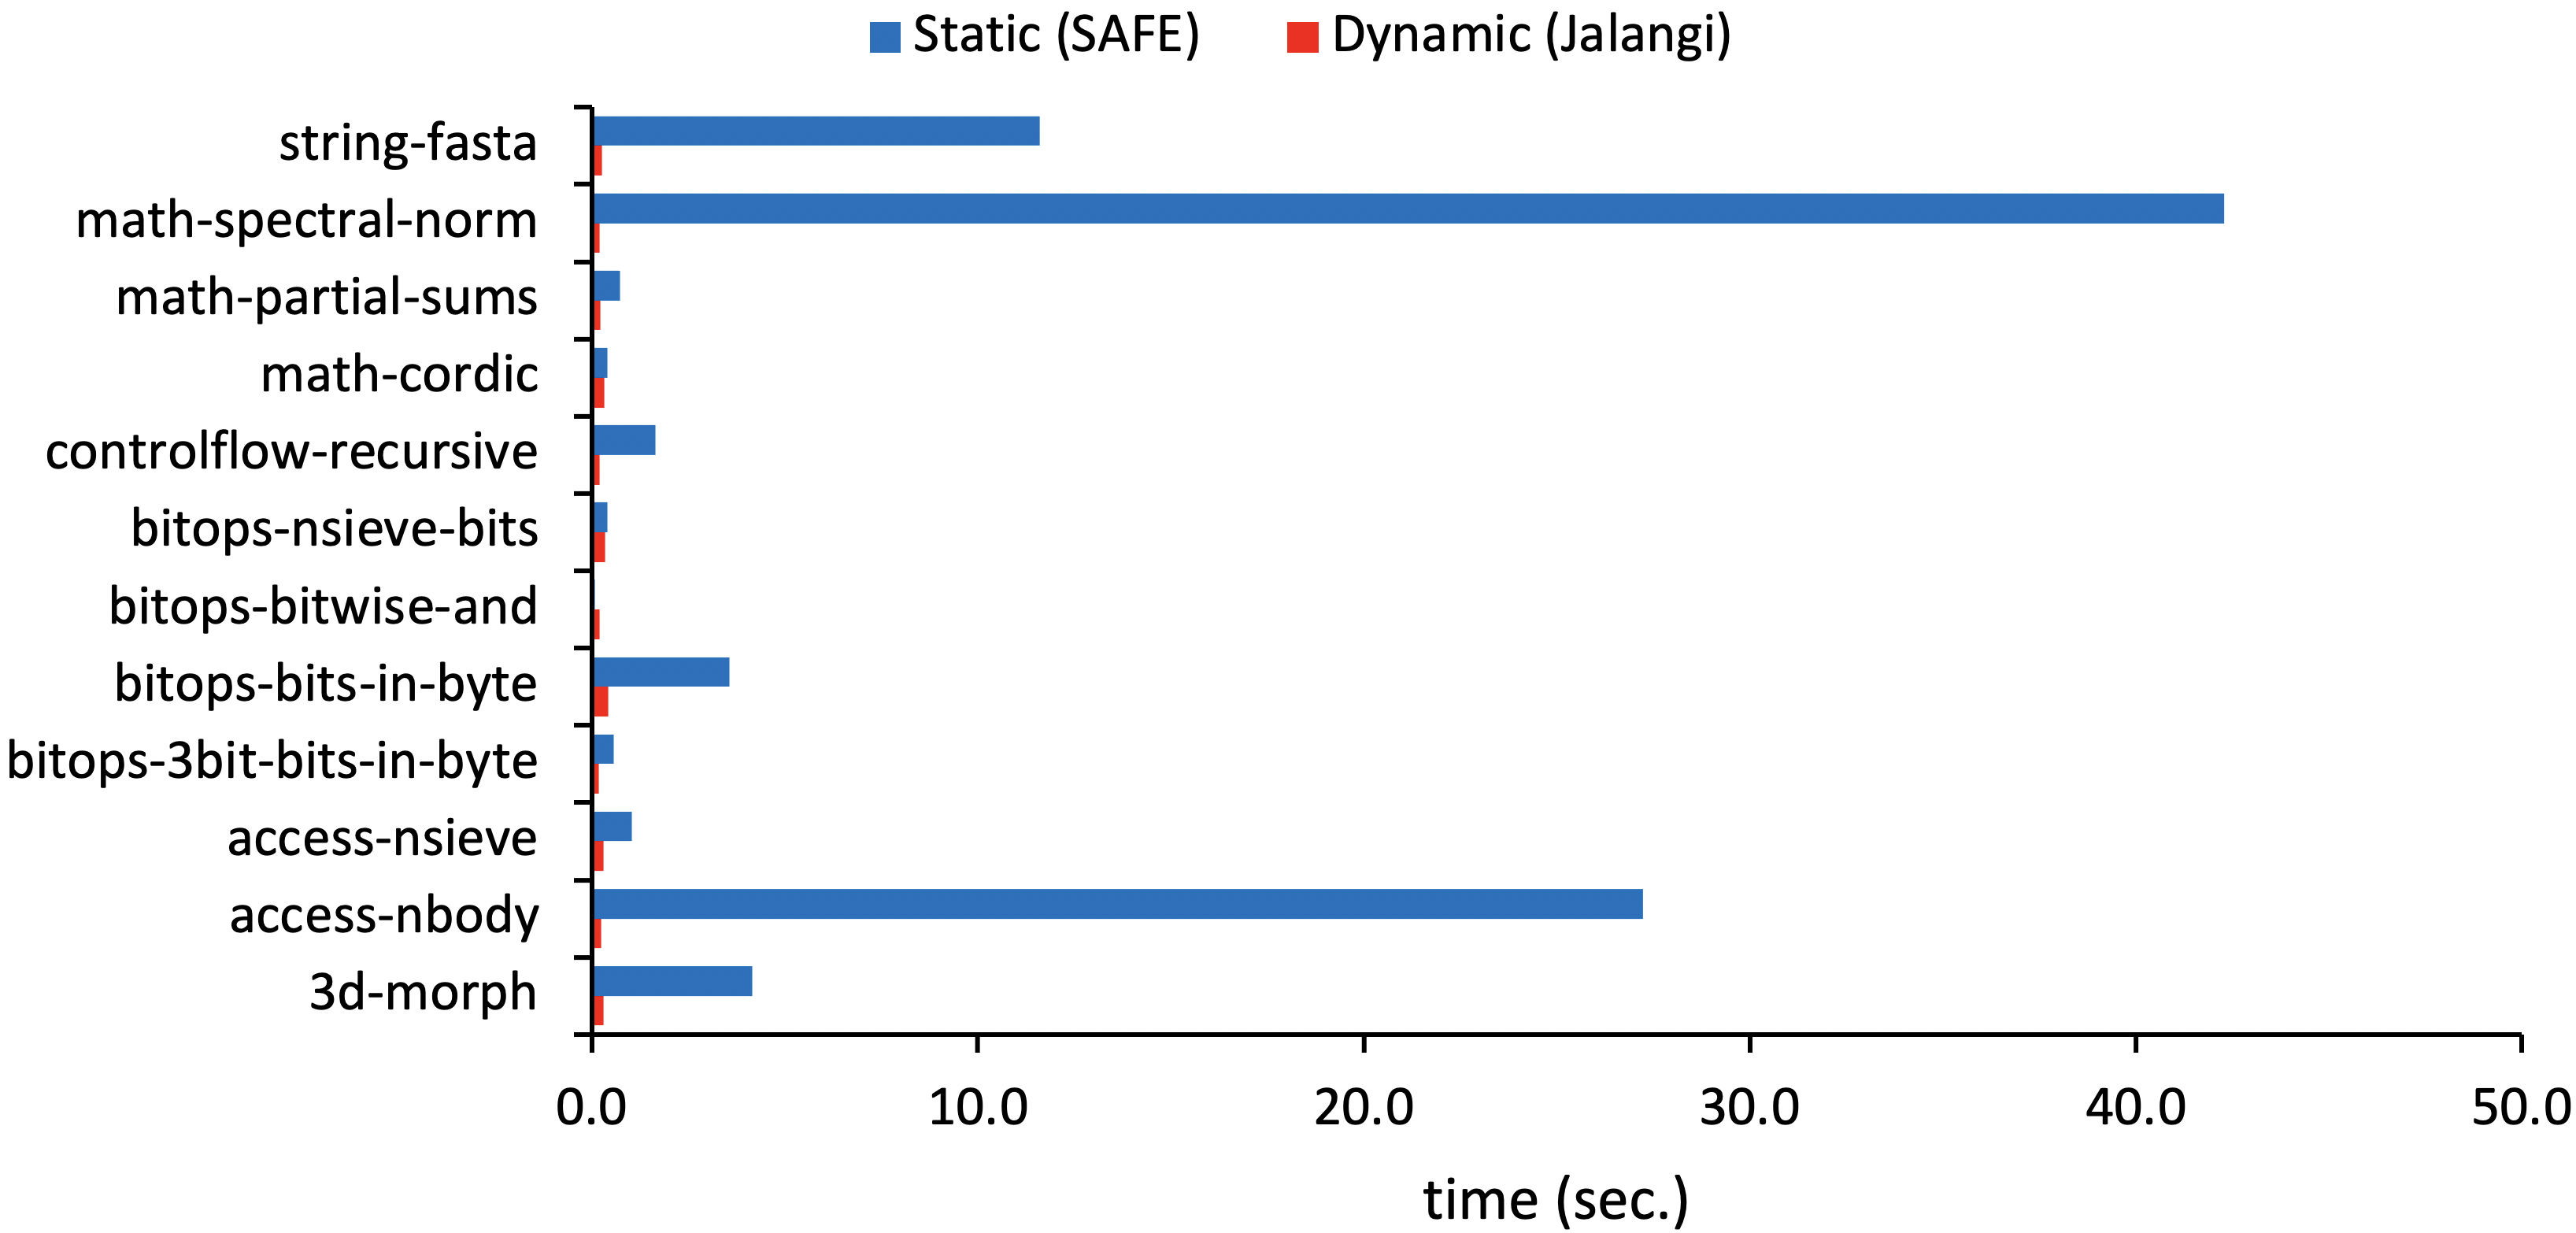
\includegraphics[width=\linewidth]{img/performance_v8v7}
  \vspace*{-2em}
  \caption{Performance of a dynamic analyzer and a static analyzer for a subset
  of the SunSpider benchmark}
  \label{fig:performance}
  \vspace*{-1em}
\end{figure}

To alleviate these problems, researchers have leveraged
dynamic analysis during static analysis.  \inred{Because dynamic
analyzers such as Jalangi~\cite{jalangi} and DLint~\cite{dlint} run on
highly-optimized commercial JavaScript engines while static analyzers run on
their own interpreters, that leads to a great gap in performance.}
Figure~\ref{fig:performance} shows that the dynamic analyzer
Jalangi is 34.8x faster than the static analyzer SAFE for a subset of the
SunSpider benchmark \inred{that is input-independent and deterministic}.
Using high performance dynamic analysis, researchers have
reduced the scope of static analysis~\cite{determinacy, blendedJS} and constructed
initial abstract states~\cite{battles, eha} and automatic modeling of opaque
code~\cite{sra}.

Unfortunately, existing techniques using dynamic analysis for static analysis
have two limitations: 1) they do not fully utilize the high performance of dynamic
analysis, and 2) they sacrifice the soundness of static analysis.  Most of
them are \textit{staged analyses}, which first extract specific
information via dynamic analysis and utilize it in static analysis.
\citet{determinacy} identify determinate expressions that always have the same
values at given program points, \citet{blendedJS} extract dynamic values to
change expressions to certain literals, and Park et al.~\cite{battles,eha} dump
the initial states of a certain host environment or the entry of an event handler.
However, because they do not utilize dynamic analysis as soon as static
analysis begins, they do not get performance benefits since then.  Moreover,
they sacrifice the soundness of static analysis by performing dynamic analysis.
For example, the SRA model~\cite{sra} uses dynamic analysis for opaque code
with abstract arguments during static analysis.  When the abstract arguments
represent an infinite number of values, it randomly samples finite
concrete values for the abstract arguments, which makes the analysis
result unsound due to missing concrete values.

In this paper, we propose a novel technique to fully utilize
the high performance of dynamic analysis for JavaScript static
analysis in a sound manner by using \textit{dynamic shortcuts}.
During static analysis, one can take a dynamic shortcut, which
consists of three parts: 1) converting the current abstract state to
its corresponding \textit{sealed symbolic state}, 2) performing
\textit{sealed symbolic execution} on the sealed symbolic state, and
3) converting the result of the sealed symbolic execution to its
corresponding abstract state.  Our key observation is that we can use
the fast concrete execution for specific program parts while
preserving the soundness if they do not use abstract values.
For example, consider static analysis of the following code:
\begin{lstlisting}[style=myJSstyle,numbers=none]
    var v = ... // an abstract value
    var obj = { p1: v }, y = "p";
    x = obj[y + 1];
\end{lstlisting}
Because \jscode{y + 1} evaluates to \jscode{"p1"},
the third line assigns the abstract value of \jscode{v} stored in
\jscode{obj.p1} to the variable \jscode{x}.
Note that even though \jscode{obj} contains an abstract value \jscode{v},
because the third line does not ``use'' the value of \jscode{v},
we can concretely execute the code.  Based on this observation,
we introduce sealed symbolic execution, which is concrete execution
using \textit{sealed symbolic values}.  A sealed symbolic value is a
representation of an abstract value in symbolic execution; it signals
the end of the current dynamic shortcut when the sealed symbolic
execution tries to access its value.
To evaluate our technique, we implemented $\tool$ using both SAFE
and Jalangi and analyzed 269 official tests of Lodash 4 library.

The contributions of this paper include the following:
\begin{itemize}
\item We present a novel technique for JavaScript static
analysis to leverage the high performance of dynamic analysis using
dynamic shortcuts.  We formally define the technique and prove
its soundness and termination.
\item We actualize the proposed technique in $\tool$, an
extended combination of SAFE and Jalangi.
\item For empirical evaluation, we analyzed 269 official tests of
Lodash 4 library.  The experiment shows that $\tool$ outperforms
SAFE 6.30$\x$ on average.  Moreover, by using dynamic shortcuts
instead of manual modeling for 12 opaque functions,
$\tool$ improves the analysis precision to detect 6 more dead branches on
average.
\end{itemize}

In the remainder of this paper, Section~\ref{sec:motivation} explains the
motivation of this work with a simple example.  Section~\ref{sec:formal}
formalizes the language-agnostic part of the technique in the abstract
interpretation framework.  Then, we extend the formalization with
JavaScript specific features in Section~\ref{sec:javascript}.
Section~\ref{sec:implementation} describes important details of the
$\tool$ implementation.  We explain the evaluation results of $\tool$
with real-world benchmarks in Section~\ref{sec:eval}.
Section~\ref{sec:related} discusses related work and
Section~\ref{sec:conclusion} concludes.

\section{Overview}

\todo

\section{Formalization}

In this section, we formally define the dynamic shortcut over the abstract
interpretation.


\subsection{Concrete Semantics}
\[
  \prog ::= (\lab: \inst)^*\\
\]
A program $\prog$ is a sequence of labelled instructions.  We represent the
semantics of a program $\prog$ as a state transition system $(\stset, \trans,
\istset)$.  A state $\st \in \stset = \labset \times \memset$ is a pair of a
label and a memory and represents a status of the program $\prog$.  A memory
$\mem \in \memset = \locset \finmap \valset$ is a finite mapping from locations
to values. A program starts with an initial state in $\istset$.  The transition
relation $\trans \subseteq \stset \times \stset$ describes how states are
transformed to other states.

A \textit{collecting semantics} $\sem{\prog} = \{ \st \in \stset \mid \ist \in
\istset \wedge \ist \trans^* \st \}$ consists of reachable states from initial
states of the program $\prog$.  We could calculate it using the \textit{transfer
function} $\transfer: \dom \rightarrow \dom$ as follows:
\[
  \sem{\prog} = \underset{n \rightarrow \infty}{\lim}{\transfer^n(\ielem)}\\
  \qquad
  \transfer(\elem) = \elem \join \step(\elem)\\
\]
The \textit{concrete domain} $\dom = \powerset{\stset}$ is a complete lattice
with $\cup$, $\cap$, and $\subseteq$ as its join($\join$), meet($\meet$), and
partial order($\order$) operators.  The initial states are $\ielem = \istset$.
The \textit{one-step execution} $\step: \dom \rightarrow \dom$ transforms states
using the transition relation $\trans$: $\step(\elem) = \{ \st' \mid \st \in
\elem \wedge \st \trans \st' \}$.


\subsection{Abstract Interpretation}
The abstract interpretation over-approximate the transfer $\transfer$ to the
\textit{abstract transfer function} $\abstransfer: \absdom \rightarrow \absdom$
to get the \textit{abstract semantics} $\abssem{\prog}$ in finite iterations as
follows:
\[
    \abssem{\prog} = \underset{n \rightarrow
    \infty}{\lim}{(\abstransfer)^n(\iabselem)}\\
\]
We define a \textit{state abstraction} $\dom \galois{\alpha}{\gamma} \absdom$ as
a Galois connection between the concrete domain $\dom$ and an abstract domain
$\absdom$ with a \textit{concretization function} $\gamma$ and a
\textit{abstraction function} $\alpha$.  The initial abstract state $\iabselem
\in \absdom$ represents an abstraction of the initial state set; $\ielem
\subseteq \gamma(\iabselem)$.  The abstract transfer function $\abstransfer:
\absdom \rightarrow \absdom$ is defined as $\abstransfer(\abselem) = \abselem
\join \absstep(\abselem)$ with an \textit{abstract one-step execution}
$\absstep: \absdom \rightarrow \absdom$.  For the sound state abstraction, the
join operator and the abstract one-step execution should satisfy the following
conditions:
\begin{itemize}
  \item $\forall \abselem_0, \abselem_1 \in \absdom. \; \gamma(\abselem_0) \cup
    \gamma(\abselem_1) \subseteq \gamma(\abselem_0 \join \abselem_1)$
  \item $\forall \abselem \in \absdom. \; \absstep \circ \gamma(\abselem) \subseteq
    \gamma \circ \absstep(\abselem)$
\end{itemize}


\subsection{Analysis Sensitivity}

Abstract interpretation is often defined with \textit{analysis sensitivity} to
increase the precision of static analysis.  A sensitive abstract domain
$\sabsdom: \viewset \rightarrow \absdom$ is defined with a \textit{view
abstraction} $\viewmap: \viewset \rightarrow \dom$ that provides multiple points
of views for reachable states during static analysis.  It maps a finite number
of views $\viewset$ to sets of states $\dom$. Each view $\view \in \viewset$
represents a set of states $\viewmap(\view)$.
A \textit{sensitive state abstraction} $\dom
\galois{\alpha_\viewmap}{\gamma_\viewmap} \sabsdom$ is a Galois connection between
the concrete domain $\dom$ and the sensitive abstract domain $\sabsdom$ with the
following concretization function:
\[
  \gamma_\viewmap(\abselem) = \{ \st \in \stset \mid \forall \view \in \viewset.
  \; \st \in \viewmap(\view) \Rightarrow \st \in \gamma \circ \sabselem(\view) \}
\]

With analysis sensitivities, the abstract one-step execution $\sabsstep:
\sabsdom \rightarrow \sabsdom$ is defined as follows:
\[
  \sabsstep(\sabselem) = \lambda \view \in \viewset. \; \underset{\view' \in
  \viewset}{\bigjoin}{\viewtrans{\view'}{\view} \circ \sabselem(\view')}
\]
where $\viewtrans{\view'}{\view}: \absdom \rightarrow \absdom$ is the abstract
semantics of a \textit{view transition} from a view $\view'$ to another view
$\view$.  It should satsify the following condition for the soundness of the
analysis:
\[
  \forall \abselem \in \absdom. \; \step(\gamma(\abselem) \cap \viewmap(\view'))
  \cap \viewmap(\view) \subseteq \gamma \circ
  \viewtrans{\view'}{\view}(\abselem)
\]

One of the most widely-used sensitivity techniques is \textit{flow sensitivity}
using a flow sensitive view abstraction $\fsviewmap: \labset \rightarrow \dom$.
It discriminates states using their labels as follows:
\[
  \forall \lab \in \labset. \; \fsviewmap(\lab) = \{ \st \in \stset \mid \st =
  (\lab, \_) \}
\]


\subsection{Abstract Counting}

We define a \textit{memory abstraction} $\powerset{\memset}
\galois{\alpha_\memset}{\gamma_\memset} \absmemset$ as a Galois connection
between sets of concrete memories and abstract memories.  An abstract memory
$\absmem \in \absmemset: \abslocset \finmap \absvalset$ is a finite mapping from
abstract locations to abstract values.  The \textit{strong update} in memory
abstraction is important to increase the precision of static analysis.  For
sound analysis, a memory update for a specific abstract location should join old
abstract values with new abstract values, which calls a \textit{weak update}.
It degrades the analysis precision because of the sprious values.  To overcome
such degradation, researchers proposed the abstract
counting~\cite{abstract-gc-counting, revisit-recency} to track how many times an
abstract location has been allocated and to apply strong updates to singleton
abstract locations.

We extended abstract states with an abstract counting operator $\abscount{-}:
\abslocset \rightarrow \abscountset = \{ \abszero, \absone, \absmany \}$, which
is a function that takes an abstract location and returns its abstract count;
$\abszero$ denotes that it have never been allocated, $\absone$ once, and
$\absmany$ more than equals to twice.


\subsection{On-Demand Access Aanlysis}

\section{Application: JavaScript}

In this section, we introduce the core language of JavaScript that supports
first-class functions, open objects, and first-class property names, and define
combined analysis of the core language.

\subsection{Core Language of JavaScript}

\begin{figure*}[t]
  \centering

  \fbox{$\st \trans \st$}
  \begin{mathpar}
    \inferrule*[width=0.48\textwidth]
    {
      \prog(\lab) = \refer = \expr\\
      \referrule{\st}{\refer}{\loc}\\
      \exprrule{\st}{\expr}{\val}\\
    }
    {
      \st = (\lab, \mem, \ctxtstack, \addr)
      \trans
      (\labnext(\lab), \mem[\loc \mapsto \val], \ctxtstack, \addr)
    }

    \inferrule*[width=0.48\textwidth]
    {
      \prog(\lab) = \refer = \kwobj\\
      \referrule{\st}{\refer}{\loc}\\
      \addr' = \text{(a fresh object address)}
    }
    {
      \st = (\lab, \mem, \ctxtstack, \addr)
      \trans
      (\labnext(\lab), \mem[\loc \mapsto \addr'], \ctxtstack, \addr)
    }

    \inferrule*[width=0.48\textwidth]
    {
      \prog(\lab) = \refer = \expr_f ( \expr_a )\\
      \referrule{\st}{\refer}{\loc}\\
      \exprrule{\st}{\expr_f}{\fval{x}{\lab_b}}\\
      \exprrule{\st}{\expr_a}{\val_a}\\
      \addr' = \text{(a fresh environment address)}
    }
    {
      \st = (\lab, \mem, \ctxtstack, \addr)
      \trans
      (\lab_b, \mem[(\addr', x) \mapsto \val_a], (\addr, \labnext(\lab), \loc)
      :: \ctxtstack, \addr')
    }

    \inferrule*[width=0.48\textwidth]
    {
      \prog(\lab) = \kwret \; \expr\\
      \exprrule{\st}{\expr}{\val}\\
    }
    {
      \st = (\lab, \mem, (\addr', \lab', \loc) :: \ctxtstack, \addr)
      \trans
      (\lab', \mem[\loc \mapsto \val], \ctxtstack, \addr')
    }

    \inferrule*[width=0.48\textwidth]
    {
      \prog(\lab) = \kwif \; \expr \; \lab'\\
      \exprrule{\st}{\expr}{\kwtrue}\\
    }
    {
      \st = (\lab, \mem, \ctxtstack, \addr)
      \trans
      (\lab', \mem, \ctxtstack, \addr)
    }

    \inferrule*[width=0.48\textwidth]
    {
      \prog(\lab) = \kwif \; \expr \; \lab'\\
      \exprrule{\st}{\expr}{\kwfalse}\\
    }
    {
      \st = (\lab, \mem, \ctxtstack, \addr)
      \trans
      (\labnext(\lab), \mem, \ctxtstack, \addr)
    }
  \end{mathpar}

  \fbox{$\referrule{\st}{\refer}{\loc}$}
  \begin{mathpar}
    \inferrule*[width=0.48\textwidth]
    {}
    {
      \referrule{\st = (\lab, \mem, \ctxtstack, \addr)}{x}{(\addr, x)}\\
    }

    \inferrule*[width=0.48\textwidth]
    {
      \exprrule{\st}{\expr_0}{\addr_0}\\
      \exprrule{\st}{\expr_1}{\val_1}\\
      \val_1 \in \strset\\
    }
    {
      \referrule{\st = (\lab, \mem, \ctxtstack, \addr)}{\expr_0 [ \expr_1
      ]}{(\addr_0, \val_1)}
    }
  \end{mathpar}

  \fbox{$\exprrule{\st}{\expr}{\val}$}
  \begin{mathpar}
    \inferrule*[width=0.48\textwidth]
    {
    }
    {
      \exprrule{\st = (\lab, \mem, \ctxtstack, \addr)}{\pval}{\pval}
    }

    \inferrule*[width=0.48\textwidth]
    {
    }
    {
      \exprrule{\st = (\lab, \mem, \ctxtstack,
      \addr)}{\fval{x}{\lab'}}{\fval{x}{\lab'}}
    }

    \inferrule*[width=0.48\textwidth]
    {
      \referrule{\st}{\refer}{\loc}\\
      \loc \in \mem\\
    }
    {
      \exprrule{\st = (\lab, \mem, \ctxtstack, \addr)}{\refer}{\mem(\loc)}
    }

    \inferrule*[width=0.48\textwidth]
    {
      \referrule{\st}{\refer}{\loc}\\
      \loc \not\in \mem\\
    }
    {
      \exprrule{\st = (\lab, \mem, \ctxtstack, \addr)}{\refer}{\kwundef}
    }

    \inferrule*[width=0.48\textwidth]
    {
      \exprrule{\st}{\expr_1}{\val_1}\\
      \cdots\\
      \exprrule{\st}{\expr_n}{\val_n}\\
    }
    {
      \exprrule{\st = (\lab, \mem, \ctxtstack, \addr)}
      {\op(\expr_1, \cdots, \expr_n)}{\op(\val_1, \cdots, \val_n)}
    }
  \end{mathpar}

  \caption{The transition relation for the core language of JavaScript}
  \label{fig:core-trans-rel}
\end{figure*}

\[
  \begin{array}{ll@{~}c@{~}l}
    \text{Programs} & \prog &::=& (\lab: \inst)^*\\

    \text{Labels} & \lab &\in& \labset\\

    \text{Instructions} & \inst &::=&
    \refer = \expr \mid
    \refer = \kwobj \mid
    \refer = \expr ( \expr ) \mid
    \kwret \; \expr \mid
    \kwif \; \expr \; \lab\\

    \text{References} & \refer &::=&
    x \mid
    \expr [ \expr ]\\

    \text{Expressions} & \expr &::=&
    \pval \mid
    \lambda x. \; \lab \mid
    \refer \mid
    \op(\expr^*)\\
  \end{array}
\]

A program $\prog$ is a sequence of labelled instructions. An instruction $\inst$
is an expression assignment, an object creation, a function call, a return
instruction, or a branch.  An expression $\expr$ is a primitive, a lambda
function, a reference, or an operation between other expressions.  A reference
$\refer$ is a variable or a property access of an object.

\[
  \begin{array}{lr@{~}c@{~}l@{~}c@{~}l}
    \text{States} & \st &\in& \stset &=& \labset \times \memset \times
    \ctxtset^* \times \eaddrset\\
    \text{Memories} & \mem &\in& \memset &=& \locset \rightarrow \valset\\
    \text{Contexts} & \ctxt &\in& \ctxtset &=& \eaddrset \times \labset \times
    \locset\\
    \text{Locations} & \loc &\in& \locset &=& (\eaddrset \times \varset) \uplus
    (\oaddrset \times \strset)\\
    \text{Values} & \val &\in& \valset &=& \pvalset \uplus \oaddrset \uplus
    \fvalset\\
    \text{Primitives} & \pval &\in& \pvalset &=& \strset \uplus \cdots\\
    \text{Addresses} & \addr &\in& \addrset &=& \eaddrset \uplus \oaddrset\\
    \text{Functions} & \fval{x}{\lab} &\in& \fvalset &=& \varset \times
    \labset\\
  \end{array}
\]

States $\stset$ consist of labels $\labset$, memories $\memset$, context stacks
$\ctxtset^*$, and environment addresses.  A memory $\mem \in \memset$ is a
mapping from locations to values.  Context stacks is sequences of contexts
$\ctxtset$ and a context $\ctxt \in \ctxtset$ is a tuple of an environment
address, a return label, and a left-hand side location.  A location $\loc \in
\locset$ is a variable or an object property; a variable location consists of an
environment address and its name, and an object property location consists of an
object address and a string value.  A value $\val \in \valset$ is a primitive,
an address, or a function value.  An address $\addr \in \addrset$ is an
environment address or an object address.  A function value
$\fval{x}{\lab}{\addr} \in \fvalset$ consists a parameter and a body label.  In
the core language, the closed scoping is used for functions for brevity thus
only parameters and local variables are accessible in the function body.

We formulate the concrete semantics of the core language as described in
Figure~\ref{fig:core-trans-rel}.  The transition relation between concrete
states is defined with the semantics of references and expressions using two
different forms \fbox{$\referrule{\st}{\refer}{\loc}$} and
\fbox{$\exprrule{\st}{\expr}{\val}$}, respectively.  The special value
$\kwundef$ denotes an undefined value and it is produced when the program access
an unknown location.


\subsection{Abstract Semantics}

\todo


\subsection{Abstract Counting}

We define a \textit{memory abstraction} $\powerset{\memset}
\galois{\alpha_\memset}{\gamma_\memset} \absmemset$ as a Galois connection
between sets of concrete memories and abstract memories.  An abstract memory
$\absmem \in \absmemset: \abslocset \finmap \absvalset$ is a finite mapping from
abstract locations to abstract values.  The \textit{strong update} in memory
abstraction is important to increase the precision of static analysis.  For
sound analysis, a memory update for a specific abstract location should join old
abstract values with new abstract values, called as a \textit{weak update}.
It degrades the analysis precision because of the sprious values.  To overcome
such degradation, researchers proposed the abstract
counting~\cite{abstract-gc-counting, revisit-recency} to track how many times an
abstract location has been allocated and to apply strong updates to singleton
abstract locations.

We extend abstract states with an abstract counting operator $\abscount{-}:
\abslocset \rightarrow \abscountset = \{ \abszero, \absone, \absmany \}$, which
is a function that takes an abstract location and returns its abstract count;
$\abszero$ denotes that it have never been allocated, $\absone$ once, and
$\absmany$ more than or equals to twice.

\section{Evaluation}\label{sec:eval}

We evaluate $\tool$ using the following research questions:
\begin{itemize}
\item \textbf{RQ1) Analysis Speed-up:} How much analysis time is reduced by
using dynamic shortcuts?
\item \textbf{RQ2) Precision Improvement:} How much analysis precision is
improved by using dynamic shortcuts?
% instead of manual modeling?
\item \textbf{RQ3) Opaque Function Coverage:} How many opaque functions are
covered only by dynamic shortcuts?
% without using manual modeling?
\end{itemize}
We selected the official 306 tests of Lodash 4
(v.4.17.20)\footnote{https://github.com/lodash/lodash/blob/4.17.20/test/test.js}
used in the examples in Section~\ref{sec:motivation} as our evaluation target.
Recent work~\cite{value-refinement,
value-partitioning} also used the tests to evaluate their techniques.
Among them, we filtered out 37 tests that use JavaScript language
features SAFE does not support such as dynamic code generation using
\njscode{Function}, getters and setters, and browser-specific features like $\jscode{__proto__}$.
Thus, we used 269 out of 306 tests for the evaluation of $\tool$.
We performed our experiments on a Ubuntu machine
equipped with 4.2GHz Quad-Core Intel Core i7 and 64GB of RAM.


\subsection{Analysis Speed-up}

\begin{figure}[t]
  \centering
  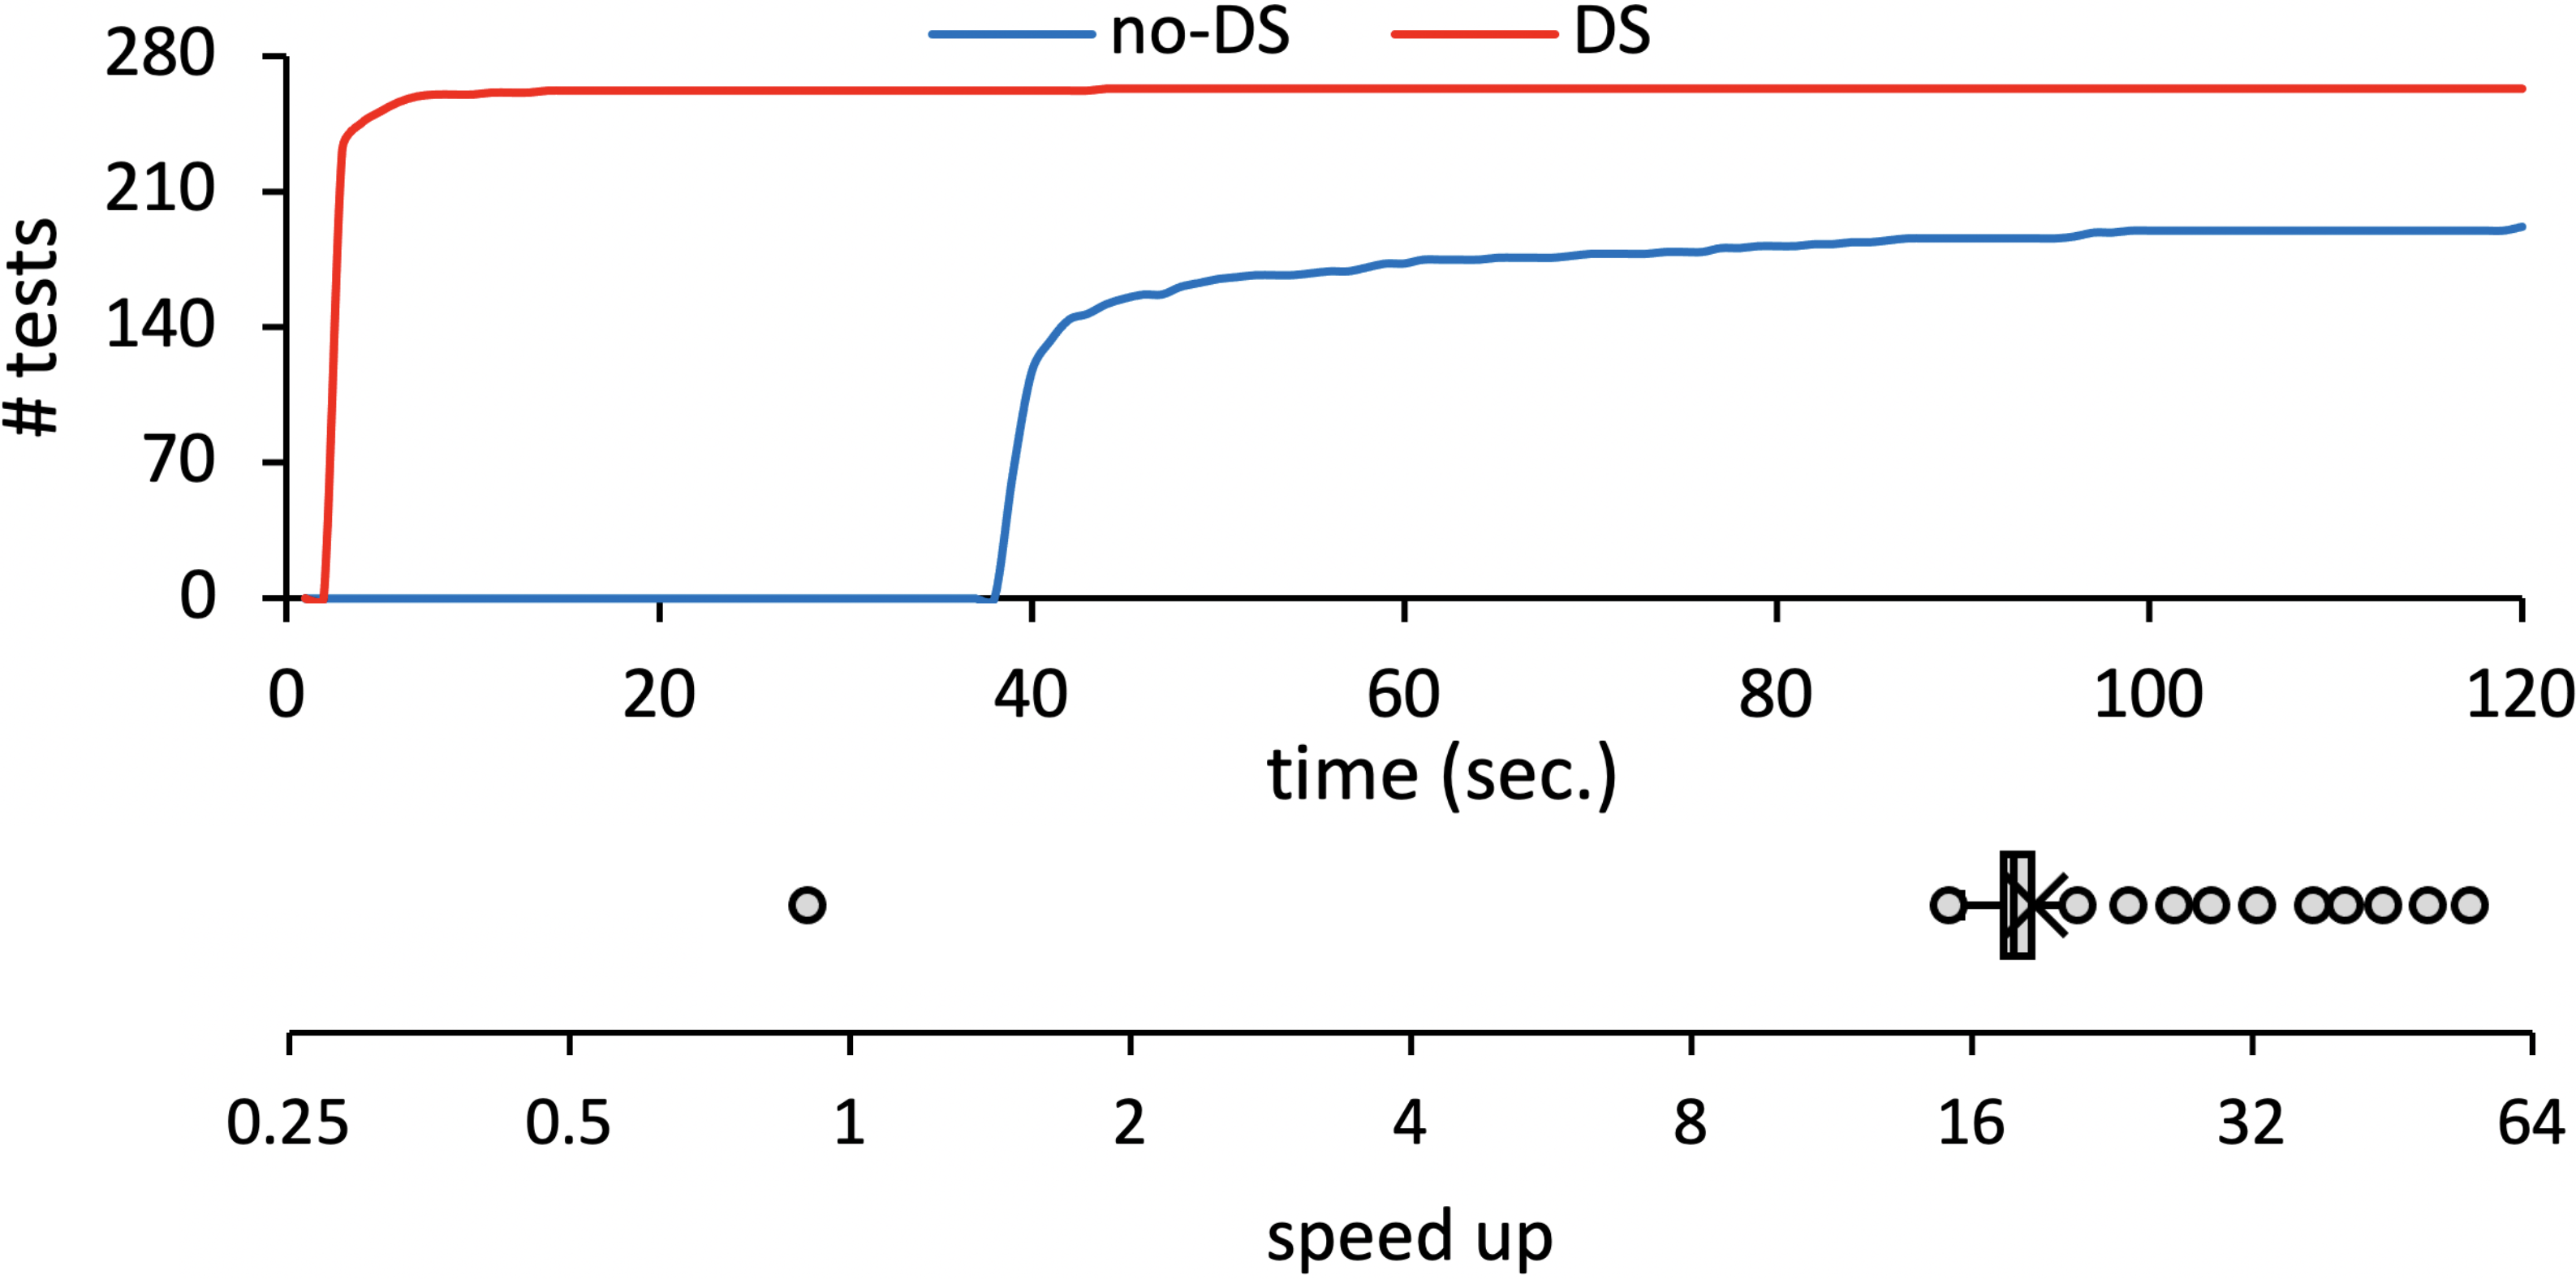
\includegraphics[width=\linewidth]{img/conc-analysis-time}
  \vspace*{-1.5em}
  \caption{Analysis time for Lodash 4 \textit{original} tests without (no-DS)
  and with (DS) dynamic shortcuts within 5 minutes}
  \label{fig:conc-analysis-time}
  \vspace*{-1.5em}
\end{figure}

\begin{figure}[t]
  \centering
  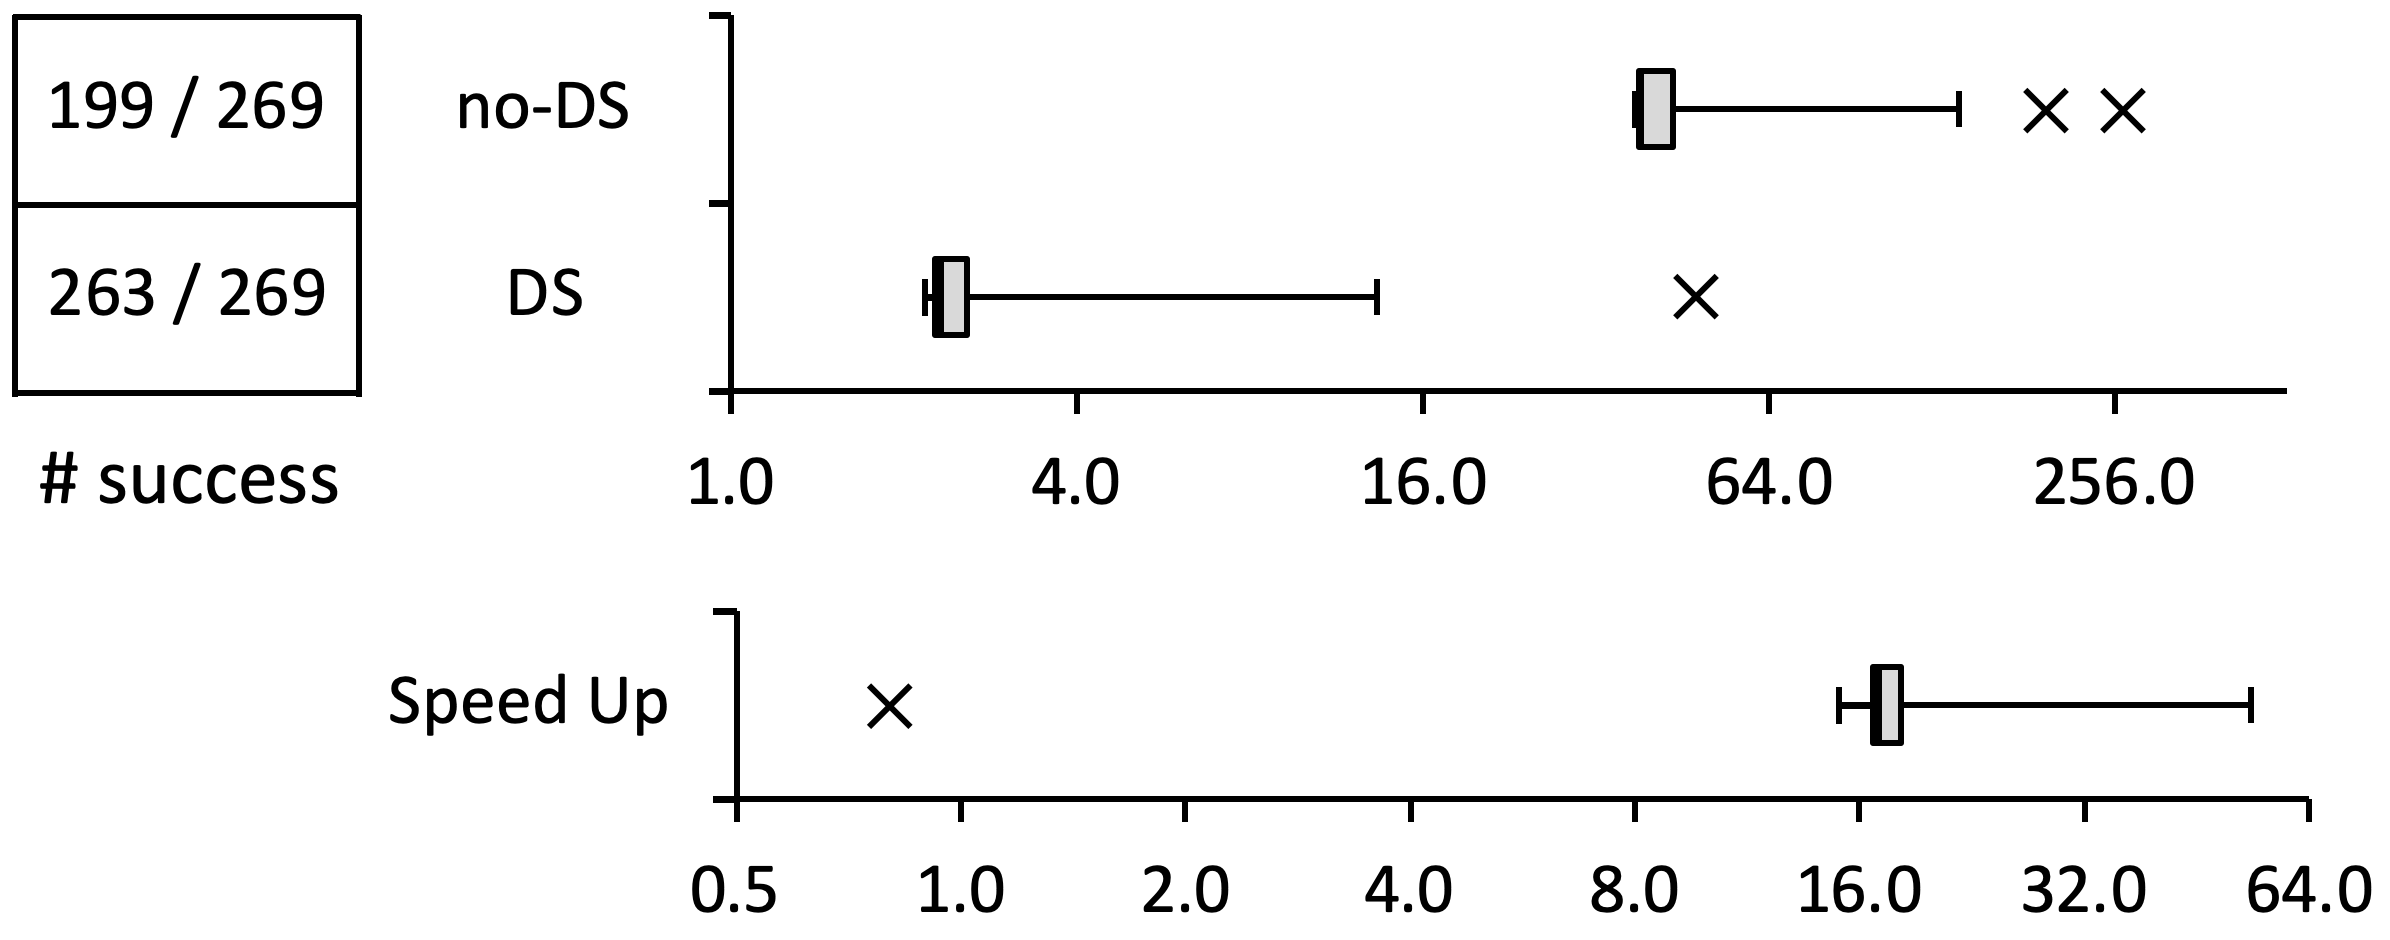
\includegraphics[width=\linewidth]{img/abs-analysis-time}
  \vspace*{-1.5em}
  \caption{Analysis time for Lodash 4 \textit{abstracted} tests without (no-DS)
  and with (DS) dynamic shortcuts within 5 minutes}
  \label{fig:abs-analysis-time}
  \vspace*{-1.5em}
\end{figure}

To evaluate the effectiveness of using dynamic shortcuts, we performed static
analysis of 269 Lodash 4 tests with and without dynamic shortcuts.
Figure~\ref{fig:conc-analysis-time} depicts cumulative distribution charts for
their analysis time and a box plot in a logarithmic scale for speed up after
applying dynamic shortcuts.  In the upper chart, the $x$-axis is time and the
$y$-axis shows the number of tests within the time.  While the baseline analysis
(no-DS) finished analysis of 200 out of 269 tests within 5 minutes, our tool
(DS) finished analysis of \inred{263} tests using dynamic shortcuts.  For finished
tests, the average analysis time is \inred{49.57} seconds for no-DS and \inred{2.78} seconds for
DS.  Among 200 tests analyzed by no-DS, \inred{two tests} are timeout in DS, thus
\inred{198} tests are analyzable by both analyzers. For them, we depict the box plot for
analysis speed up by dynamic shortcuts.  It shows that DS
outperforms no-DS up to \inred{54.98$\x$} and \inred{19.96$\x$} on
average.  Only for one test using $\jscode{_.sample}$, which
randomly samples a value from a given array, DS showed
\inred{0.90$\x$ speed of no-DS due to 24 times uses} of dynamic shortcuts.

Note that since most tests use concrete values instead of
non-deterministic inputs, they can be analyzed by a few number of dynamic shortcuts.
In fact, among 269 tests, \inred{262} tests are analyzed
by a single dynamic shortcut without using abstract semantics.
However, in real-world JavaScript programs, arguments of library
functions may include non-deterministic inputs.
To evaluate $\tool$ in a real-world setting,
we modified the tests to use abstract values.
We made abstract values by randomly selecting literals and replacing
one of them with its corresponding abstract value.
For example, if we select a numeric literal \jscode{42}, we modified it to the abstract numeric value
$\top_{\code{num}}$, which represents all the numeric values.
In the remaining section, we evaluated $\tool$ using the \textit{original} tests
and the \textit{abstracted} tests.

For abstracted tests as well, DS outperformed no-DS.
Figure~\ref{fig:abs-analysis-time} shows the analysis time of the abstracted tests.
Among 269 abstracted tests, no-DS finished analysis of 158 tests within 5 minutes,
but DS finished analysis of \inred{167} tests.  For finished tests, the average analysis
time is \inred{44.88} seconds for no-DS and \inred{42.28} seconds for DS. Among 158 tests analyzed by no-DS, DS
timed-out for \inred{15} tests.  For \inred{143} tests analyzable by both analyzers,
DS outperformed no-DS up to \inred{50.60$\x$} and \inred{6.30$\x$} on average.
\inred{Except for 6 test cases, using dynamic shortcut did show speed up.}

\begin{figure}[t]
  \centering
  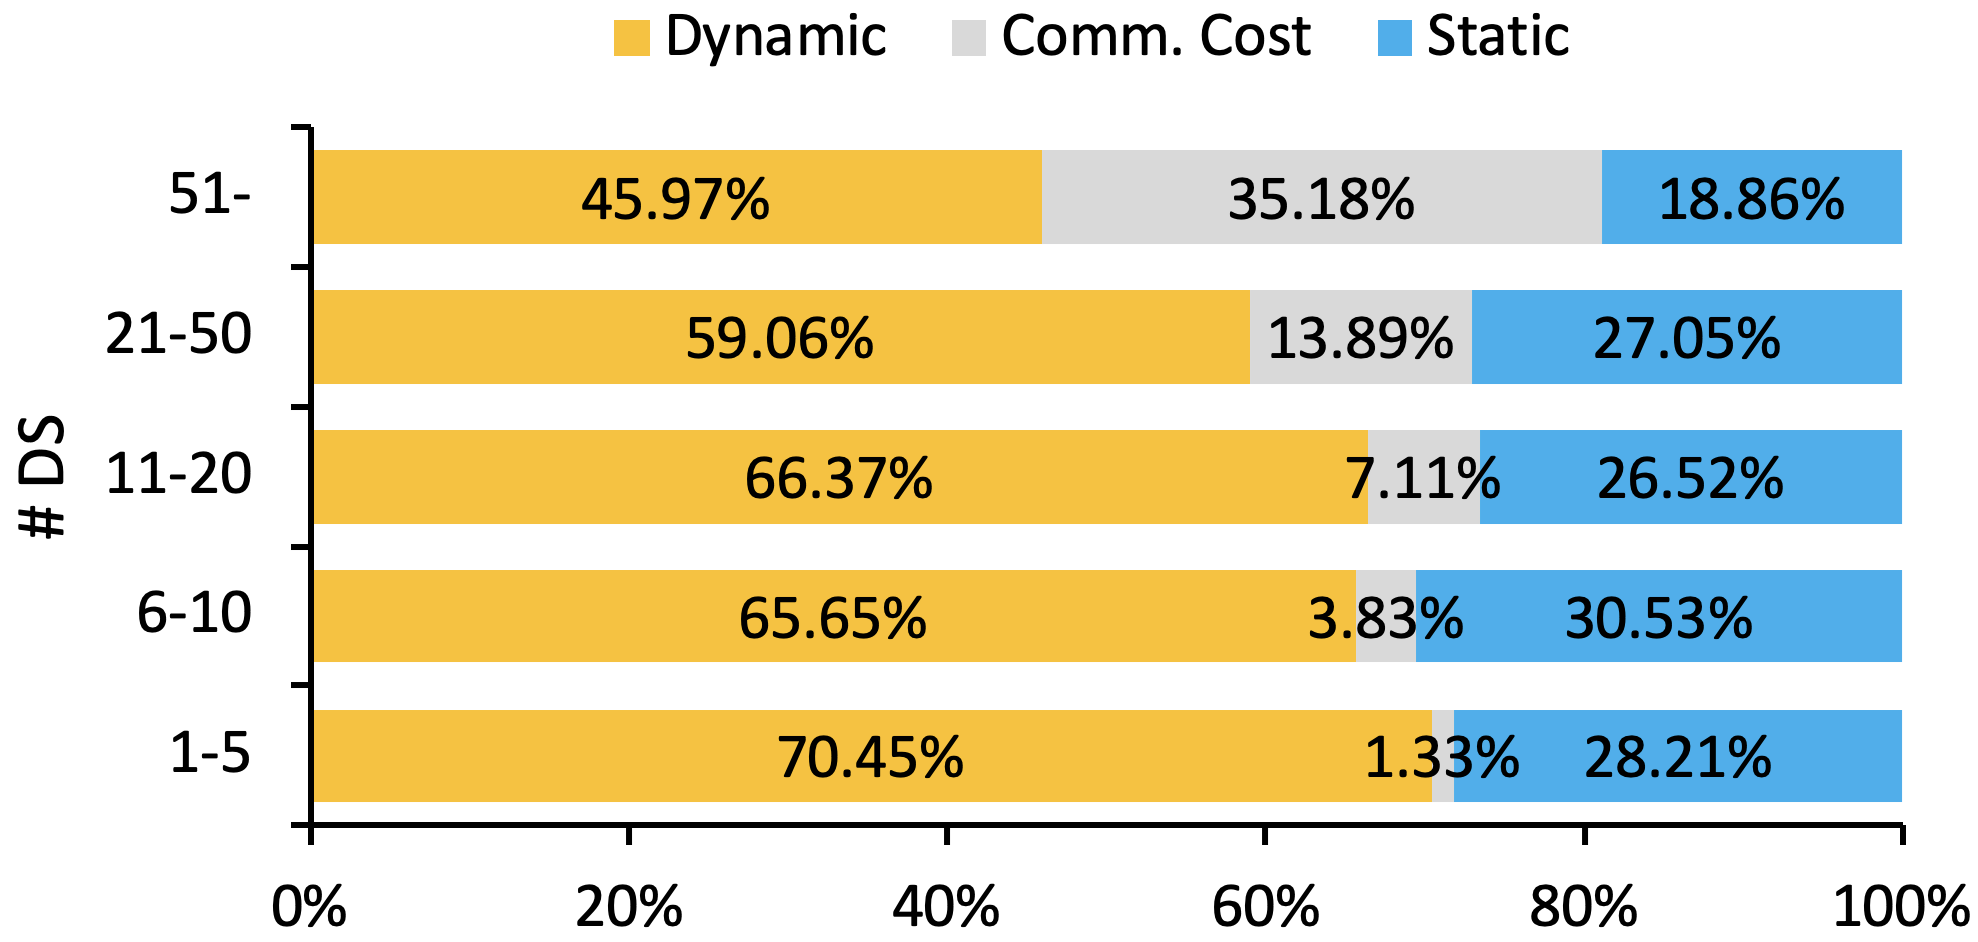
\includegraphics[width=\linewidth]{img/abs-analysis-ratio}
  \vspace*{-1.5em}
  \caption{Analysis time ratio for \inred{143} \textit{abstracted} tests}
  \label{fig:abs-analysis-ratio}
  \vspace*{-1.5em}
\end{figure}

\begin{table*}[t]
  \caption{Number of original (orig.) and abstracted (abs.) tests using dynamic shortcuts
only for each JavaScript built-in library}
  \label{table:func-replace}
  \vspace*{-1em}
  \centering
  \scriptsize
  \[
\quad
    \begin{array}{c|l|c|c?c|l|c|c?c|l|c|c}

      \myhead{Object}       {Function}        {\# Replaced}

      \mysutf{1}{}          {Array    }  {203 / 203}{ 90 / 116} & \mysutf{1}{}             {String     }  { 20 /  20}{  9 /  10} & \mysutf{1}{}       {Object        }  {263 / 263}{151 / 167} \mylinefff
      \mysutf{1}{}          {new Array}  {  0 /   0}{  0 /  10} & \mysutf{1}{}             {toString   }  {  0 /   0}{  0 /  33} & \mysutf{1}{}       {new Object    }  {  0 /   0}{  0 /   3} \mylinefff
      \mysutf{1}{}          {isArray  }  {263 / 263}{144 / 167} & \mysutf{1}{}             {valueOf    }  {  0 /   0}{  0 /  12} & \mysutf{1}{}       {getPrototypeOf}  { 56 /  56}{ 24 /  29} \mylinefff
      \mysutf{1}{}          {concat   }  {263 / 263}{163 / 167} & \mysutt{1}{}             {charAt     }  {  7 /   7}{  5 /   5} & \mysutf{1}{}       {create        }  {263 / 263}{164 / 167} \mylinefff
      \mysutf{1}{}          {join     }  {263 / 263}{166 / 167} & \mysutf{1}{}             {charCodeAt }  { 15 /  15}{  3 /   4} & \mysutf{1}{Object} {defineProperty}  {263 / 263}{160 / 167} \mylinefff
      \mysutf{1}{}          {pop      }  { 25 /  25}{  9 /  13} & \mysutt{1}{}             {indexOf    }  {  2 /   2}{  1 /   1} & \mysbtt{1}{}       {freeze        }  {  1 /   1}{  1 /   1} \mylinefff
      \mysutf{2}{Array}     {push     }  {263 / 263}{150 / 167} & \mysutf{1}{String}       {match      }  { 25 /  25}{ 11 /  13} & \mysutf{1}{}       {keys          }  {263 / 263}{161 / 167} \mylinefff
      \mysutt{1}{}          {reverse  }  { 10 /  10}{  3 /   3} & \mysutf{1}{}             {replace    }  { 55 /  55}{ 19 /  26} & \mysutf{1}{}       {toString      }  {263 / 263}{129 / 167} \mylinefff
      \mysutf{1}{}          {shift    }  {  2 /   2}{  0 /   1} & \mysutf{1}{}             {slice      }  {263 / 263}{165 / 167} & \mysutf{1}{}       {hasOwnProperty}  {263 / 263}{161 / 167} \mylinefft
      \mysutf{1}{}          {slice    }  {263 / 263}{164 / 167} & \mysutf{1}{}             {split      }  {  5 /   5}{  0 /   1} & \mysutf{1}{}       {parseInt}        {  1 /   1}{  0 /   1} \mylinefff
      \mysutf{1}{}          {sort     }  { 69 /  69}{ 26 /  28} & \mysutf{1}{}             {substring  }  {214 / 214}{ 91 / 121} & \mysutf{1}{Global} {isNaN   }        { 15 /  15}{  9 /  25} \mylinefff
      \mysutf{1}{}          {splice   }  { 25 /  25}{  6 /  11} & \mysutf{1}{}             {toLowerCase}  {214 / 214}{ 90 / 121} & \mysbtt{1}{}       {isFinite}        {  3 /   3}{  1 /   1} \mylinefft
      \mysutt{1}{}          {unshift  }  {  2 /   2}{  1 /   1} & \mysutf{1}{}             {toUpperCase}  { 10 /  10}{  4 /   6} & \mysbtt{1}{}       {RegExp    }      {263 / 263}{167 / 167} \mylineftf
      \mysutf{1}{}          {indexOf  }  { 94 /  94}{ 22 /  47} & \mysutt{2}{Boolean}      {Boolean}      {  3 /   3}{  2 /   2} & \mysutf{2}{RegExp} {new RegExp}      {  0 /   0}{  0 /   1} \mylinefff
      \mysutf{1}{}          {every    }  { 92 /  92}{ 23 /  32} & \mysutf{1}{}             {valueOf}      {  0 /   0}{  0 /   6} & \mysbtt{1}{}       {exec      }      {263 / 263}{167 / 167} \mylinettf
      \mysutt{1}{}          {ceil }      { 36 /  36}{  8 /   8} & \mysutf{2}{Number}       {Number }      {  2 /   2}{  1 /   2} & \mysutf{1}{}       {test      }      {263 / 263}{158 / 167} \mylinefft
      \mysuff{1}{}          {floor}      { 16 /  17}{  4 /   5} & \mysutf{1}{}             {valueOf}      {  0 /   0}{  0 /  16} & \mysutf{1}{}       {Error         }  {  1 /   1}{  0 /   1} \mylineftf
      \mysutf{1}{Math}      {max  }      {263 / 263}{134 / 167} & \mysutt{1}{}             {toString}     {263 / 263}{167 / 167} & \mysutf{2}{Error}  {new Error     }  {  0 /   0}{  0 /   8} \mylinefff
      \mysutf{1}{}          {min  }      { 64 /  64}{ 15 /  48} & \mnsutf{1}{Function}     {apply   }     {263 / 263}{124 / 167} & \mysutf{1}{}       {new RangeError}  {  0 /   0}{  0 /   3} \mylinefff
      \mysutt{1}{}          {pow  }      { 11 /  11}{  5 /   5} & \mysuff{1}{}             {call    }     {262 / 263}{ 50 / 167} & \mysutf{1}{}       {new TypeError }  {  0 /   0}{  0 /   9}
    \end{array}
  \]
  \vspace*{-1em}
\end{table*}

Unlike for the original tests, analysis of \inred{143} abstracted tests invoked
\inred{16.05} dynamic shortcuts.  Because taking a dynamic shortcut
requires conversion between abstract states and {\sealed} values
and their exchanges between the static analyzer and the dynamic analyzer,
using dynamic shortcuts multiple times may incur more performance
overhead than performance benefits by using {\sealed} execution.
One conjecture is that the communication cost between the static
analyzer and the dynamic analyzer may be proportional to the number of
dynamic shortcuts.

To experimentally evaluate the conjecture, we investigated the relationship between
the communication cost between analyzers and the number of dynamic shortcuts.
For \inred{198} original tests, the communication cost was only
\inred{3.51\%} compared to the analysis time of no-DS.  However, for \inred{143}
abstracted tests, the communication cost was \inred{82.49\%} compared to the analysis
time of no-DS.  Figure~\ref{fig:abs-analysis-ratio} presents the
analysis time ratio for \inred{143} abstracted tests.
The $x$-axis represents the time ratio normalized by the total analysis time of
no-DS and the $y$-axis denotes the number of dynamic
shortcuts and the number of corresponding tests.
For all \inred{143} tests, the communication cost (Comm. Cost) is larger than
both the static analysis time (Static) and the dynamic analysis
time (Dynamic).  When dynamic shortcuts are performed less than 10 times,
the communication cost is modest compared with the baseline static
analysis time.  However, the more dynamic shortcuts are performed,
the less the performance benefits by using dynamic shortcuts.
\inred{Specifically, when dynamic shortcuts are performed more than
20 times, Comm. Cost is even larger than no-DS.}
Based on this evaluation result, we believe that we can leverage
dynamic shortcuts by optimizing the communication cost between
the static analyzer and the dynamic analyzer.

\begin{figure}[t]
  \centering
  \begin{subfigure}[t]{0.48\textwidth}
    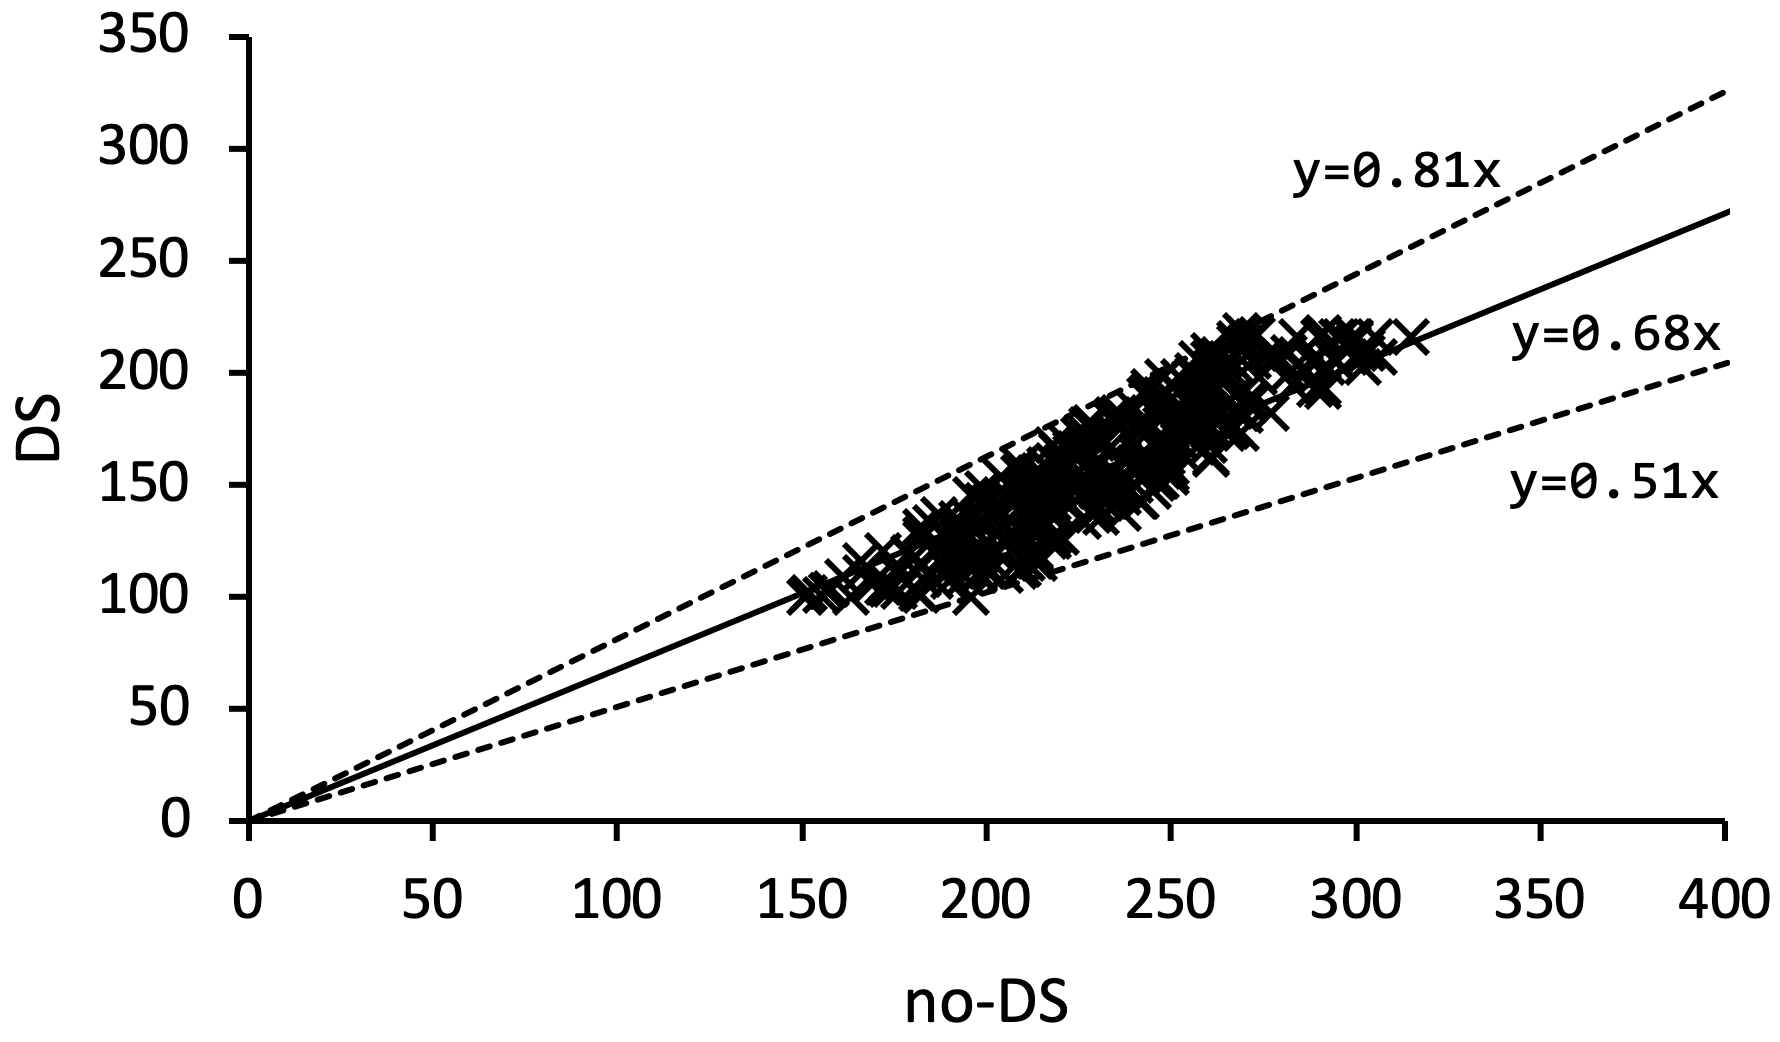
\includegraphics[width=\linewidth]{img/conc-precision}
    \vspace*{-1.5em}
    \caption{Reachable branches for \inred{198} \textit{original} tests}
    \label{fig:precision-fail}
  \end{subfigure}
  \begin{subfigure}[t]{0.48\textwidth}
    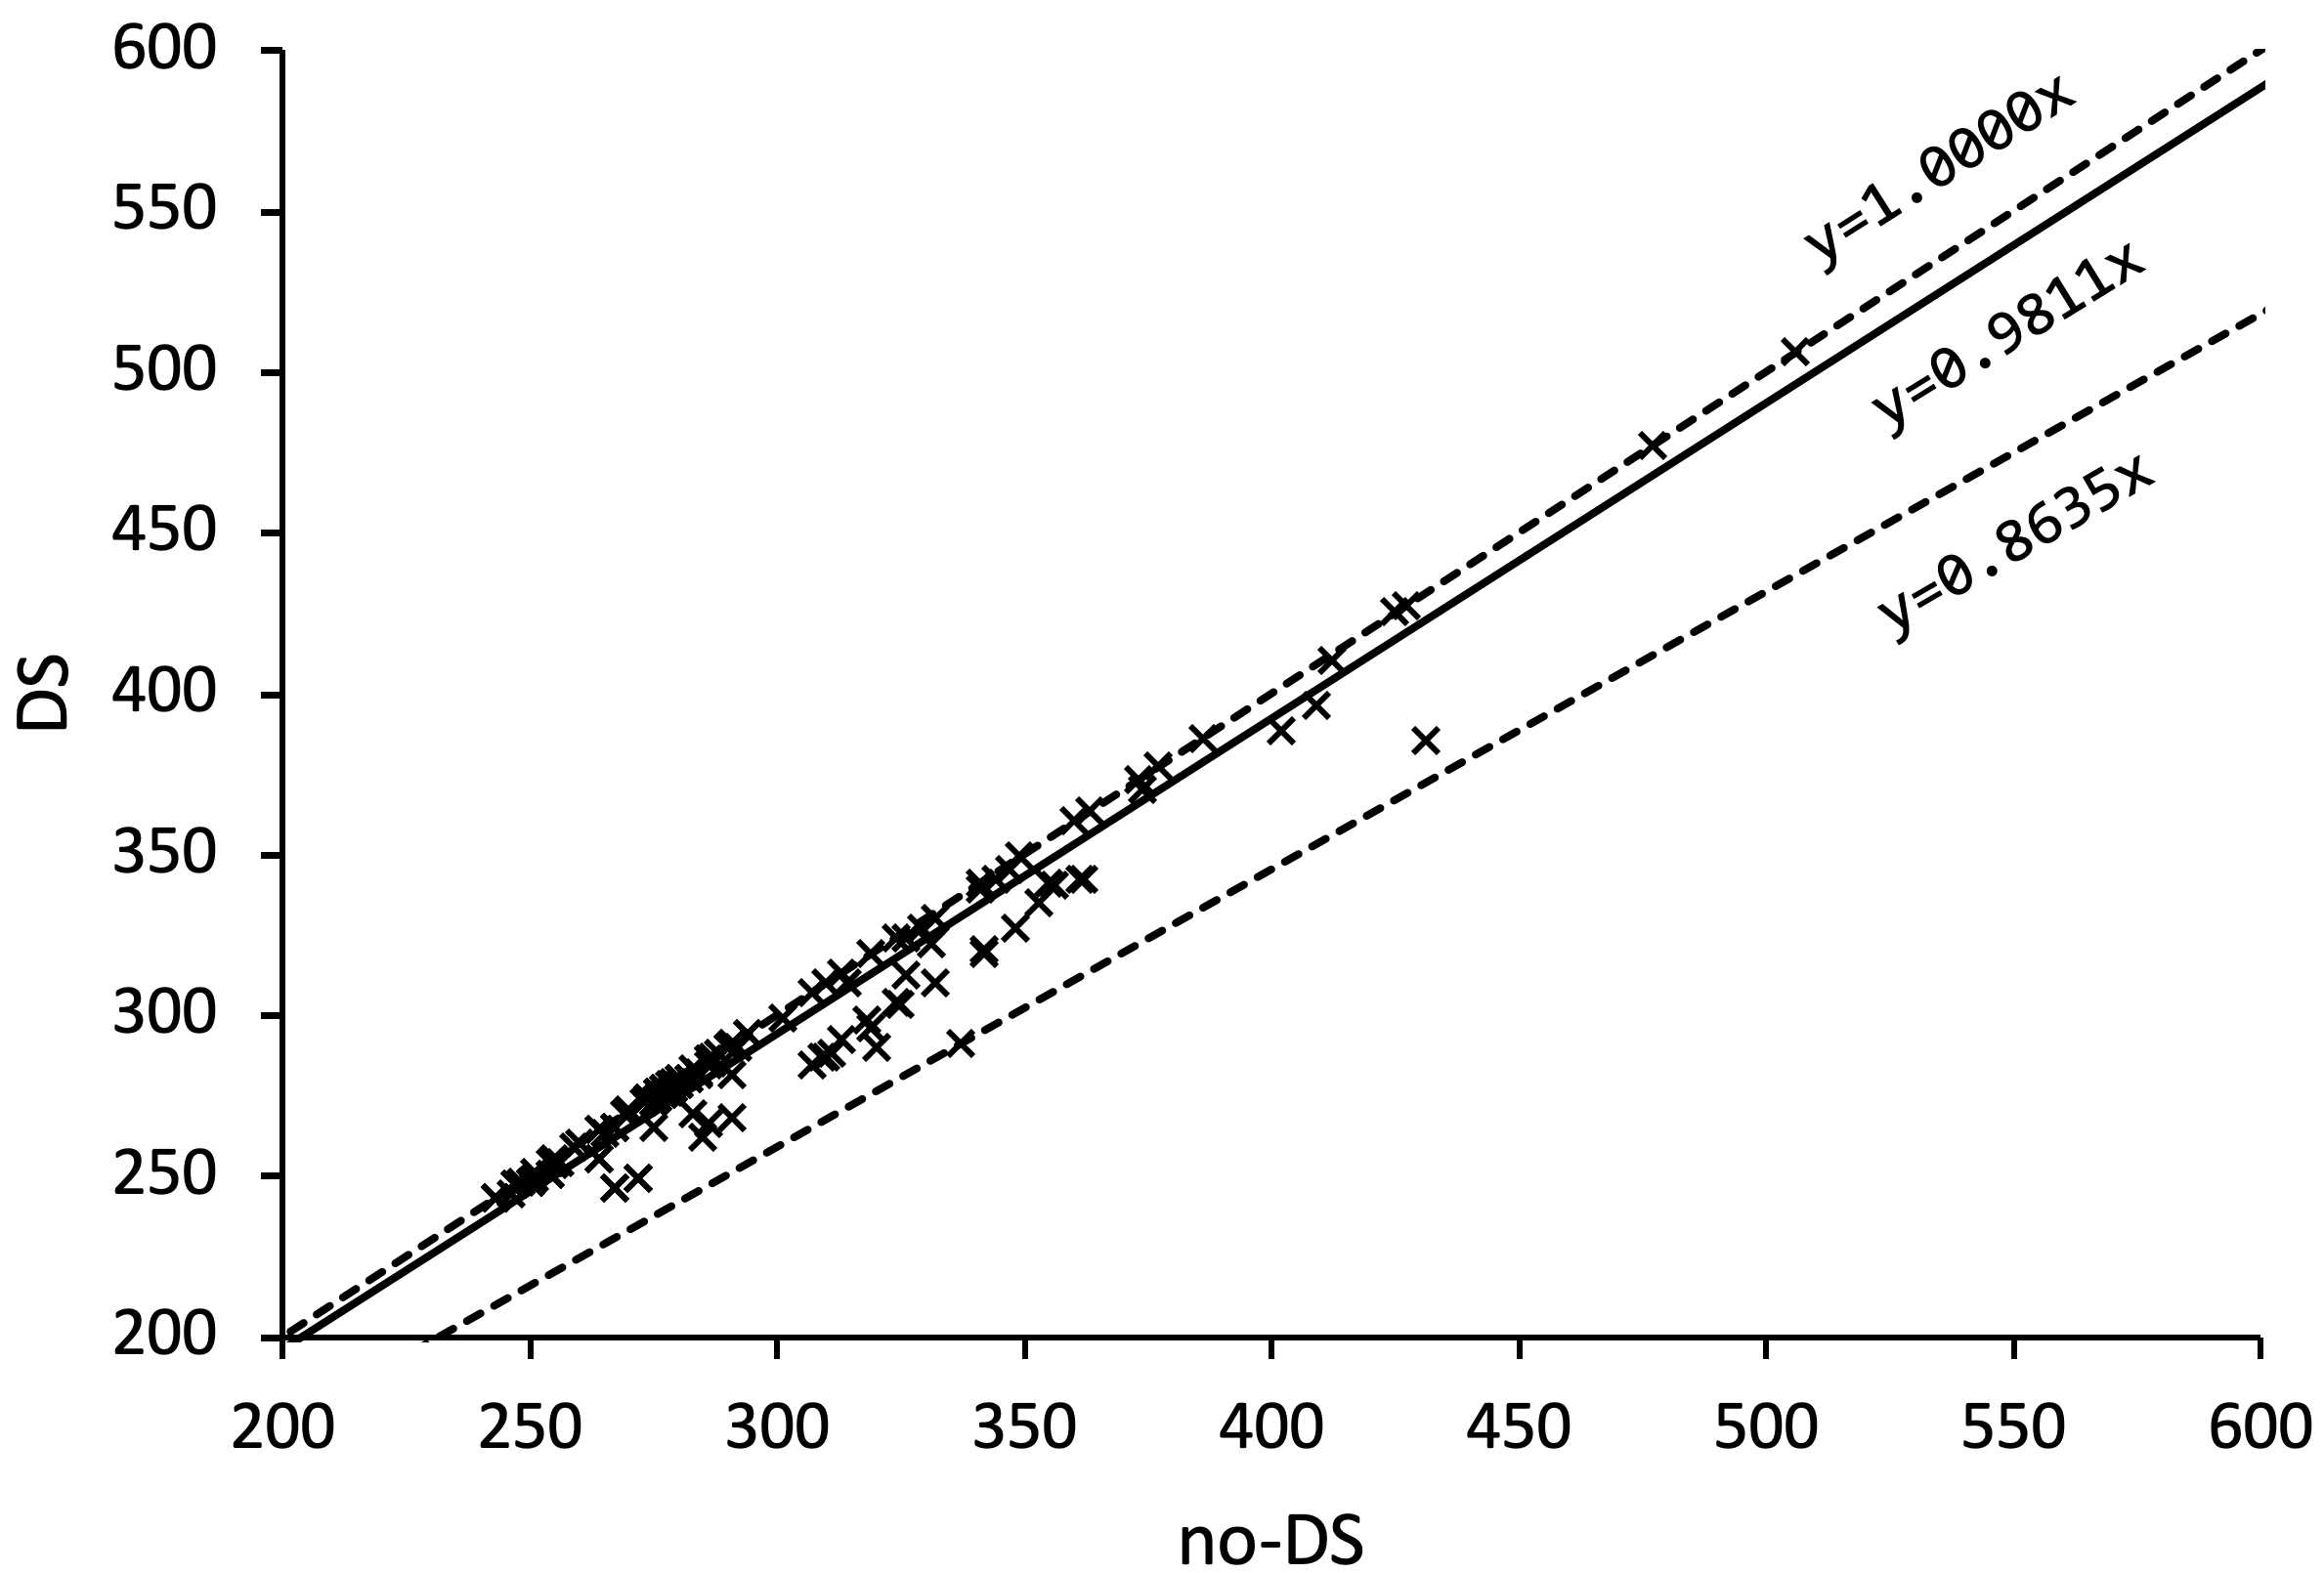
\includegraphics[width=\linewidth]{img/abs-precision}
    \vspace*{-1.5em}
    \caption{Reachable branches for \inred{143} \textit{abstracted} tests}
    \label{fig:precision-branch}
  \end{subfigure}
  \vspace*{-1em}
  \caption{Branch coverage of analysis without (no-DS) and with (DS) dynamic shortcuts}
  \label{fig:precision}
  \vspace*{-1.5em}
\end{figure}



\subsection{Precision Improvement}

To evaluate the analysis precision improvement of dynamic shortcuts,
we measured the number of \inred{assertion fails invoked by} no-DS and DS.
Because both no-DS and DS are sound,
high (low) \inred{number of assertion fails} denotes low (high) analysis precision.

Figure~\ref{fig:precision} depicts the comparison of the analysis
precision between no-DS and DS.  The $x$-axis and the $y$-axis denote
the number of \inred{assertion fails invoked} by no-DS and DS, respectively;
each \inred{circle} mark denotes each test \inred{in heatmap form. The darker the circle is, the more tests it indicates.} The top line
denotes the y=x line, and
the bottom solid line denotes the average improvement.
For \inred{198} original tests that are analyzable by both analyzers,
Figure~\ref{fig:precision}(a) shows that dynamic shortcuts
\inred{completely removed the assertion fails for 24 tests, reducing the nuber of assertion fails by 93\% on average.}
For \inred{143} abstracted tests that are analyzable by both analyzers,
Figure~\ref{fig:precision}(b) shows that dynamic shortcuts successfully cut down
the number of \inred{covered branches 12\% on average.}
Thus, on average, dynamic shortcuts removed analysis of \inred{93\%} and \inred{12\%} spurious alarms
for original and abstracted tests, respectively.

\section{Related Work}\label{sec:related}

Several researchers have introduced analysis technique to utilize dynamic
analysis for static analysis in three different ways: combined analysis,
automatic modeling, and pruning states.


\paragraph{Combined Analysis}

The most related previous work is the combined analysis that utilizes dynamic
analysis during Java static analysis introduced by \citet{concerto}.  They
proved that their combined analysis is sound and showed that it could
significantly improve the precision and performance of Java static analysis by
evaluating their tool, \concerto.  However, their approach have several
limitations compared to the dynamic shortcut.  First, they syntactically divides
a given program to \textit{applications} parts for static analysis and
\textit{frameworks} parts for dynamic analysis.  Thus, it is impossible to
freely switching between static and dynamic and even impossible to perform both
of static and dynamic analysis to the same program part in different contexts.
Besides, they introduced \textit{mostly-concrete interpretation} similar with
our sealed symbolic execution.  However, it supports only a special
\textit{unknown} value that represents any possible value.  Thus, it cannot
preserves the precision of complex abstract domains~\cite{safe, tajs, regex,
weaklySPE} frequently used in JavaScript static analysis.  In the other hand,
the sealed symbolic execution automatically detects whether the abstract
semantics for abstract values.  Finally, \concerto preserves the soundness when
the program satisfies the \textit{state separation hypothesis}.  They assume
that states of application and framework parts do not interrogated or
manipulated by each other.  While it is reasonable for static analysis of Java
applications using external libraries, the assumption is not satisfied for
JavaScript programs in general.  Unlike their approach, our approach does not
have any assumption between static and dynamic analysis parts.


\paragraph{Automatic Modeling}
For static analysis of JavaScript programs, modeling behaviors of built-in
libraries or host-dependent functions is required because they are opaque
codes.  Since manual modeling is error-prone, tedious, and labor-intensive,
several researchers~\cite{safewapi, safets} utilize type information to
automatically model their behaviors.  However, type information is too imprecise
to reflect the detailed semantics and is difficult to represent the
side-effects.  To alleviate the problem, \citet{mimic} introduced the technique
to infer JavaScript codes for opaque codes using concrete execution.  They
captured the effects of opaque codes on user objects by collecting partial
execution traces and synthesized JavaScript codes based on the extracted
behaviors.  They also leveraged ES6 \jscode{Proxy} objects to capture the
effects on user objects.  Instead of synthesizing JavaScript codes,
\citet{opaque-model} presented a \textit{Sample-Run-Abstract (SRA)} approach for
on-demand modeling thus they focused on the current abstract state during static
analysis.  It first \textit{samples} concrete states in a well-distributed way,
\textit{runs} each sampled state on a JavaScript engine, and \textit{abstract}
executions results.  However, all of previous works sacrifice the soundness of
static analysis.  On the other hand, while the dynamic shortcut is not
applicable for all invocation of opaque functions, it is sound if it is
applicable.


\paragraph{Pruning Analysis Scopes}
Another approach to utilize dynamic analysis for JavaScript static analysis is
to prune the scope of analysis.  \citet{blended} introduced \textit{blended
taint analysis} that specializes JavaScript dynamic language features such as
dynamic code generation (e.g. \jscode{eval}) or variadic function calls.  They
first performs dynamic analysis to collect traces with concrete values used in
dynamic language features and restrict the semantics of features based on the
collected traces during static analysis.  \citet{battles, eha} utilizes three
different points to reduce analysis scopes: initial states, dynamically loaded
files, and event handlers.  They dumped the initial states from a specific web
browser to focus on analyzing the behaviors of web browsers running on the
browser.  Then, they collected paths of dynamically loaded files via concrete
executions and utilized the path information in static analysis.  For event
handlers, they intentionally analyzed partial execution flows using concrete
user events.  They collected concrete states for each entry of event handler
during dynamic analysis, merged them to a single abstract state, and analyzed
the event handler with the abstract state.  Unfortunately, all of them does not
preserve soundness of static analysis unlike the dynamic shortcut.


% \subsection{Abstract Counting}
% 
% \begin{itemize}
%   \item Improving flow analyses via $\Gamma$CFA: Abstract garbage collection and
%     counting~\cite{abstract-gc-counting}
%   \item Revisiting recency abstraction for JavaScript: towards an intuitive,
%     compositional, and efficient heap abstraction~\cite{revisit-recency}
% \end{itemize}

% \subsection{Access Analysis}
% 
% \begin{itemize}
%   \item Access Analysis-Based Tight Localization of Abstract
%     Memories~\cite{func-local}
%   \item Design and implementation of sparse global analyses for C-like
%     languages~\cite{sparse}
% \end{itemize}

\section{Conclusion}\label{sec:conclusion}
We presented a novel technique for JavaScript static analysis using \textit{dynamic shortcuts}.
It can significantly accelerate static
analysis by freely leveraging high performance of dynamic analysis for
concretely executable program parts.  To maximize such benefits,
we proposed \textit{sealed symbolic execution}, which performs
concrete execution using sealed symbolic values for abstract values.
We formally defined static analysis using dynamic shortcuts in the
abstract interpretation framework and proved its soundness and termination.
We developed $\tool$ as a prototype implementation of the proposed approach
by extending a combination of the state-of-the-art static and dynamic
analyzers SAFE and Jalangi.  Our tool accelerates the speed
of static analysis \inred{19.96}x for original tests and \inred{6.30}x for
abstracted tests of Lodash 4 library.  Moreover, it detects \inred{6} more
dead branches by using sealed symbolic execution instead of
manual modeling for \inred{12} opaque functions on average.


\bibliographystyle{ACM-Reference-Format}
\bibliography{ref}

\end{document}
\endinput
